%% LyX 2.5.1 created this file.  For more info, see https://www.lyx.org/.
%% Do not edit unless you really know what you are doing.
\documentclass[journal,article,submit,pdftex,moreauthors]{Definitions/mdpi}
\usepackage[utf8]{inputenc}
\synctex=-1
\usepackage[dvipsnames]{xcolor}
\usepackage{colortbl}
\usepackage{array}
\usepackage{float}
\usepackage{url}
\usepackage{varwidth}
\usepackage{graphicx}

\makeatletter

%%%%%%%%%%%%%%%%%%%%%%%%%%%%%% LyX specific LaTeX commands.

\Title{Predicting Football Match Outcomes Using Machine Learning }

\Author{Morfis Sallis$^{1}$, George Georgoulas$^{2}$ and Ioannis G. Tsoulos$^{3,*}$}


\address{$^{1}$\quad{} Department of Informatics and Telecommunications,
University of Ioannina, 45500 Ioannina, Greece; e.sallis@uoi.gr\\
$^{2}$\quad{} Department of Mechanical Engineering and Aeronautics,
University of Patras, Panepistimioupoli Patron, Rio 26504, Greece;
georgoul@gmail.com\\
$^{3}\quad$ Department of Informatics and Telecommunications, University
of Ioannina, 45500 Ioannina, Greece; itsoulos@uoi.gr}


\corres{Correspondence: itsoulos@uoi.gr}


\abstract{Football match outcomes are influenced by a complex interplay of
dynamic team strategies and stochastic match events, posing a significant
challenge for predictive analytics. In this paper we present a unified
benchmarking study for football match outcome classification, using
a dataset of 225,474 matches spanning 2018-2026 and a strictly chronological
train-test split. Six classifiers spanning several modelling approaches,
Logistic Regression, Generalized Additive Models, FastTree, Random
Forest, Radial Basis Function networks and Multi-Layer Perceptron,
are trained and evaluated under identical conditions. Bookmaker odds
are converted into margin-free probabilities by the power method,
with the exponent found by Newton-Raphson, and are included among
the input features. In addition to the six classifiers we also report
a majority-class baseline and the de-vigged bookmaker prediction itself.
Results are reported for both a binary one-vs-rest formulation and
the original three-class (1, X, 2) formulation, with 95\% bootstrap
CIs for every metric and every model. Across the six classifiers the
differences are small: macro-averaged precision ranges from 64.83\%
to 65.16\% for Home Win and from 68.05\% to 68.46\% for Away Win,
and macro-averaged recall from 63.16\% to 63.51\% and from 59.10\%
to 59.72\% respectively, with substantially overlapping confidence
intervals. In the three-class formulation, models trained without
market data reach 48.0\% accuracy against 43.4\% for a trivial baseline
and 51.9\% for the bookmaker. Models trained with market data match
the bookmaker but do not improve upon it on log-loss, Brier score
or the ranked probability score.\textbf{ The only statistically distinguishable
improvement of any kind is a 0.086 point accuracy advantage for the
additive model, which is not accompanied by any improvement in the
proper scoring rules and therefore does not indicate a practical advantage.}
Probability calibration and betting-signal generation are outside
the scope of this study.}


\keyword{Machine learning; classification; sports forecasting; model benchmarking;
probability estimation.}

\DeclareTextSymbolDefault{\textquotedbl}{T1}
%% Because html converters don't know tabularnewline
\providecommand{\tabularnewline}{\\}
%% Variable width box for table cells
\newenvironment{cellvarwidth}[1][t]
    {\begin{varwidth}[#1]{\linewidth}}
    {\@finalstrut\@arstrutbox\end{varwidth}}

%%%%%%%%%%%%%%%%%%%%%%%%%%%%%% User specified LaTeX commands.
\setlength{\tabcolsep}{5pt}
%  LaTeX support: latex@mdpi.com
%  For support, please attach all files needed for compiling as well as the log file, and specify your operating system, LaTeX version, and LaTeX editor.
%=================================================================
%\documentclass[preprints,article,submit,pdftex,moreauthors]{Definitions/mdpi}
% For posting an early version of this manuscript as a preprint, you may use "preprints" as the journal. Changing "submit" to "accept" before posting will remove line numbers.
% Below journals will use APA reference format:
% admsci, aieduc, behavsci, businesses, econometrics, economies, education, ejihpe, famsci, games, humans, ijcs, ijfs, jintelligence, journalmedia, jrfm, jsam, languages, peacestud, psycholint, publications, tourismhosp, youth
% Below journals will use Chicago reference format:
% arts, genealogy, histories, humanities, laws, literature, religions, risks, socsci
%--------------------
% Class Options:
%--------------------
%----------
% journal
%----------
% Choose between the following MDPI journals:
% accountaudit, acoustics, actuators, addictions, adhesives, admsci, adolescents, aerobiology, aerospace, agriculture, agriengineering, agrochemicals, agronomy, ai, aichem, aieduc, aieng, aimater, aimed, aipa, air, aisens, algorithms, allergies, alloys, amh, analog, analytica, analytics, anatomia, anesthres, animals, antibiotics, antibodies, antioxidants, applbiosci, appliedchem, appliedmath, appliedphys, applmech, applmicrobiol, applnano, applsci, aquacj, architecture, arm, arthropoda, arts, asc, asi, astronautics, astronomy, atmosphere, atoms, audiolres, automation, axioms, bacteria, batteries, bdcc, behavsci, beverages, biochem, bioengineering, biologics, biology, biomass, biomechanics, biomed, biomedicines, biomedinformatics, biomimetics, biomolecules, biophysica, bioresourbioprod, biosensors, biosphere, biotech, birds, blockchains, bloods, blsf, brainsci, breath, buildings, businesses, cancers, carbon, cardio, cardiogenetics, cardiovascmed, catalysts, cells, ceramics, challenges, chemengineering, chemistry, chemosensors, chemproc, children, chips, cimb, civileng, cleantechnol, climate, clinbioenerg, clinpract, clockssleep, cmd, cmtr, coasts, coatings, colloids, colorants, commodities, complexities, complications, compounds, computation, computers, condensedmatter, conservation, constrmater, cosmetics, covid, crops, cryo, cryptography, crystals, csmf, ctn, culture, curroncol, cyber, dairy, data, ddc, dentistry, dermato, dermatopathology, designs, devices, dhi, diabetology, diagnostics, dietetics, digital, disabilities, diseases, diversity, dna, drones, dynamics, earth, ebj, ecm, ecologies, econometrics, economies, edm, education, eesp, ejihpe, electricity, electrochem, electronicmat, electronics, encyclopedia, endocrines, energies, eng, engproc, entomology, entropy, environments, environremediat, epidemiologia, epigenomes, esa, est, famsci, fermentation, fibers, fintech, fire, fishes, fluids, foods, forecasting, forensicsci, forests, fossstud, foundations, fractalfract, fuels, future, futureinternet, futurepharmacol, futurephys, futuretransp, galaxies, games, gases, gastroent, gastrointestdisord, gastronomy, gels, genealogy, genes, geographies, geohazards, geomatics, geometry, geosciences, geotechnics, geriatrics, germs, glacies, grasses, green, greenhealth, gucdd, hardware, hazardousmatters, healthcare, hearts, hemato, hematolrep, hep, heritage, higheredu, highthroughput, histories, horticulturae, hospitals, humanities, humans, hydrobiology, hydrogen, hydrology, hydropower, hygiene, idr, iic, ijcs, ijem, ijerph, ijfs, ijgi, ijmd, ijms, ijns, ijom, ijpb, ijt, ijtm, ijtpp, ime, immuno, informatics, information, infrastructures, inorganics, insects, instruments, inventions, iot, j, jaestheticmed, jal, jcdd, jcm, jcp, jcrm, jcs, jcto, jdad, jdb, jdream, jemr, jeta, jfb, jfmk, jgbg, jgg, jimaging, jintelligence, jlpea, jmahp, jmmp, jmms, jmp, jmse, jne, jnt, jof, joi, joitmc, joma, jop, joptm, jor, journalmedia, jox, jpbi, jphytomed, jpm, jrfm, jsam, jsan, jtaer, jvd, jzbg, kidneydial, kinasesphosphatases, knowledge, labmed, laboratories, lae, land, languages, laws, life, lights, limnolrev, lipidology, liquids, literature, livers, logics, logistics, lubricants, lymphatics, machines, macromol, magnetism, magnetochemistry, make, marinedrugs, materials, materproc, mathematics, mca, measurements, medicina, medicines, medsci, membranes, merits, metabolites, metals, meteorology, methane, metrics, metrology, micro, microarrays, microbiolres, microelectronics, micromachines, microorganisms, microplastics, microwave, minerals, mining, mmphys, modelling, molbank, molecules, mps, msf, mti, multimedia, muscles, nanoenergyadv, nanomanufacturing, nanomaterials, ncrna, ndt, network, neuroglia, neuroimaging, neurolint, neurosci, nitrogen, notspecified, nursrep, nutraceuticals, nutrients, obesities, occuphealth, oceans, ohbm, onco, optics, oral, organics, organoids, osteology, oxygen, pandemics, parasites, parasitologia, particles, pathogens, pathophysiology, peacestud, pediatrrep, pets, pharmaceuticals, pharmaceutics, pharmacoepidemiology, pharmacy, philosophies, photochem, photonics, phycology, physchem, physics, physiologia, plants, plasma, platforms, pollutants, polymers, polysaccharides, populations, poultry, powders, precipitation, precisoncol, preprints, proceedings, processes, prosthesis, proteomes, psf, psychiatryint, psychoactives, psycholint, publications, purification, quantumrep, quaternary, qubs, radiation, rdt, reactions, realestate, receptors, recycling, regeneration, religions, remotesensing, reports, reprodmed, resources, rheumato, risks, rjpm, robotics, rsee, ruminants, safety, sci, scipharm, sclerosis, seeds, sensors, separations, sexes, shi, signals, sinusitis, siuj, skins, smartcities, sna, societies, socsci, software, soilsystems, solar, solids, spectroscj, sports, standards, stats, std, stratsediment, stresses, surfaces, surgeries, suschem, sustainability, symmetry, synbio, systems, tae, targets, taxonomy, technologies, telecom, test, textiles, thalassrep, therapeutics, thermo, timespace, tomography, tourismhosp, toxics, toxins, tph, transplantology, transportation, traumacare, traumas, tri, tropicalmed, universe, urbansci, uro, vaccines, vehicles, venereology, vetsci, vibration, virtualworlds, viruses, vision, waste, water, welding, wem, wevj, wild, wind, women, world, youth, zoonoticdis
%---------
% article
%---------
% The default type of manuscript is "article", but can be replaced by:
% abstract, addendum, article, book, bookreview, briefreport, casereport, comment, commentary, communication, conferenceproceedings, correction, conferencereport, entry, expressionofconcern, extendedabstract, datadescriptor, editorial, essay, erratum, hypothesis, interestingimage, obituary, opinion, projectreport, reply, retraction, review, perspective, protocol, shortnote, studyprotocol, systematicreview, supfile, technicalnote, viewpoint, guidelines, registeredreport, tutorial
% supfile = supplementary materials
%----------
% submit
%----------
% The class option "submit" will be changed to "accept" by the Editorial Office when the paper is accepted. This will only make changes to the frontpage (e.g., the logo of the journal will get visible), the headings, and the copyright information. Also, line numbering will be removed. Journal info and pagination for accepted papers will also be assigned by the Editorial Office.
%------------------
% moreauthors
%------------------
% If there is only one author the class option oneauthor should be used. Otherwise use the class option moreauthors.
%---------
% pdftex
%---------
% The option pdftex is for use with pdfLaTeX. If eps figures are used, remove the option pdftex and use LaTeX and dvi2pdf.
%=================================================================
% MDPI internal commands - do not modify
\firstpage{1}
\setcounter{page}{\@firstpage}
\pubvolume{1}
\issuenum{1}
\articlenumber{0}
\pubyear{2026}
\copyrightyear{2026}
%\externaleditor{Firstname Lastname} % More than 1 editor, please add `` and '' before the last editor name
\datereceived{}
\daterevised{ } % Comment out if no revised date
\dateaccepted{}
\datepublished{}
%\datecorrected{} % For corrected papers include a "Corrected: XXX" date in the original paper.
%\dateretracted{} % For retracted papers include a "RETRACTED: XXX" date in the original paper.
%\doinum{} % Used for some special journals, like molbank
%\pdfoutput=1 % Uncommented for upload to arXiv.org
%\CorrStatement{yes}  % For updates
%\longauthorlist{yes} % For many authors that exceed the left citation part
%\IsAssociation{yes} % For association journals
%=================================================================
% Add packages and commands here. The following packages are loaded in our class file: fontenc, inputenc, calc, indentfirst, fancyhdr, graphicx, epstopdf, lastpage, ifthen, lineno, float, amsmath, setspace, enumitem, mathpazo, booktabs, titlesec, etoolbox, tabto, xcolor, soul, multirow, microtype, tikz, totcount, changepage, attrib, upgreek, cleveref, amsthm, hyphenat, natbib, hyperref, footmisc, url, geometry, newfloat, caption
%=================================================================
%% Please use the following mathematics environments: Theorem, Lemma, Corollary, Proposition, Characterization, Property, Problem, Example, ExamplesandDefinitions, Hypothesis, Remark, Definition, Notation, Assumption
%% For proofs, please use the proof environment (the amsthm package is loaded by the MDPI class).
%=================================================================
% The fields PACS, MSC, and JEL may be left empty or commented out if not applicable
%\PACS{J0101}
%\MSC{}
%\JEL{}
%%%%%%%%%%%%%%%%%%%%%%%%%%%%%%%%%%%%%%%%%%
% Only for the journal Diversity
%\LSID{\url{http://}}
%%%%%%%%%%%%%%%%%%%%%%%%%%%%%%%%%%%%%%%%%%
% Only for the journal Applied Sciences:
%\featuredapplication{Authors are encouraged to provide a concise description of the specific application or a potential application of the work. This section is not mandatory.}
%%%%%%%%%%%%%%%%%%%%%%%%%%%%%%%%%%%%%%%%%%
%%%%%%%%%%%%%%%%%%%%%%%%%%%%%%%%%%%%%%%%%%
% Only for the journal Data:
%\dataset{DOI number or link to the deposited data set in cases where the data set is published or set to be published separately. If the data set is submitted and will be published as a supplement to this paper in the journal Data, this field will be filled by the editors of the journal. In this case, please make sure to submit the data set as a supplement when entering your manuscript into our manuscript editorial system.}
%\datasetlicense{license under which the data set is made available (CC0, CC-BY, CC-BY-SA, CC-BY-NC, etc.)}
%%%%%%%%%%%%%%%%%%%%%%%%%%%%%%%%%%%%%%%%%%
% Only for the journal BioTech, Fishes, Neuroimaging and Toxins
%\keycontribution{The breakthroughs or highlights of the manuscript. Authors can write one or two sentences to describe the most important part of the paper.}
%%%%%%%%%%%%%%%%%%%%%%%%%%%%%%%%%%%%%%%%%%
% Only for the journal Encyclopedia
%\encyclopediadef{Instead of the abstract}
%\entrylink{The Link to this entry published on the encyclopedia platform.}
%%%%%%%%%%%%%%%%%%%%%%%%%%%%%%%%%%%%%%%%%%
%%%%%%%%%%%%%%%%%%%%%%%%%%%%%%%%%%%%%%%%%%
% Different journals have different requirements. Please check the specific journal guidelines in the "Instructions for Authors" on the journal's official website.
%\addhighlights{yes}
%\renewcommand{\addhighlights}{%
%
%\noindent The goal is to increase the discoverability and readability of the article via search engines and other scholars. Highlights should not be a copy of the abstract, but a simple text allowing the reader to quickly and simplified find out what the article is about and what can be cited from it. Each of these parts should be devoted up to 2 bullet points.\vspace{3pt}\\
%\textbf{What are the main findings?}
% \begin{itemize}[labelsep=2.5mm,topsep=-3pt]
% \item First bullet.
% \item Second bullet.
% \end{itemize}\vspace{3pt}
%\textbf{What are the implications of the main findings?}
% \begin{itemize}[labelsep=2.5mm,topsep=-3pt]
% \item First bullet.
% \item Second bullet.
% \end{itemize}
%}
%%%%%%%%%%%%%%%%%%%%%%%%%%%%%%%%%%%%%%%%%%

\makeatother

\begin{document}
\maketitle

\section{Introduction}

Machine learning (ML) methods are now applied across a wide range
of scientific and applied fields, from the physical sciences \citep{physics_ml1,physics_ml2,astronomy_ml1,astronomy_ml2,chemistry_ml1,chemistry_ml2}
to medicine \citep{med_ml1,med_ml2} and economics \citep{econ_ml1,econ_ml2},
and the tools most often used, neural networks (NNs) \citep{nn1,nn2,nn_image,nn_timeseries},
decision trees (DTs) \citep{dt1,dt2} and support vector machines
(SVMs) \citep{svm1,svm2}. In this research study, we address the
problem of predicting the outcome of a football match by examining
it through a variety of ML techniques. This problem has been addressed
in a number of earlier studies. 

Predicting football match outcomes is difficult because of the high
levels of noise, changing team strategies, and unpredictable match
events. Standard predictive models often struggle in these volatile
environments. This research is important for three main reasons. First,
we conduct a rigorous comparative analysis. Instead of focusing on
just one algorithm, we compare different classifiers on the same input
space. This provides a controlled comparison of how each model handles
the non-linearity and volatility of sports data. Second, we report
results for both a binary one-vs-rest decomposition and the original
three-class outcome, using metrics that do not depend on an arbitrary
decision threshold. Third, and central to this study, we evaluate
all models against the de-vigged bookmaker forecast. Because market
prices already aggregate team strength, recent form and public information,
a benchmark that omits them cannot establish whether a model contributes
new information or simply reproduces the bookmaker's choice \citep{forrest2005,dixoncoles1997}.
Reporting such a comparison also calls for restraint in what is claimed
from model outputs, a concern documented in forecasting settings beyond
sport \citep{kliger2025}.

For example, Hvattum et al. proposed the incorporation of ELO ratings
for the prediction of match outcomes in their study \citep{elo_football}.
Also, Owramipur et al. used Bayesian networks \citep{ml_bayesian}
to predict the outcomes for the Spanish League Barcelona team \citep{bayesian_football}.
Similarly, Prasetio et al. proposed the incorporation of logistic
regression \citep{ml_logistic} to predict the outcomes of football
matches \citep{logistic_football}. Moreover, Martins et al. used
a polynomial classifier for the prediction of football outcomes \citep{polynomial_football}.
Schauberger et al. selected the method of random forests (RFs) to
predict the results of football matches in their study \citep{rf_football}.
Player-level attributes were studied by Danisik et al. for the same
purpose \citep{attr_football}. Constantinou proposed a new ML model,
named Dolores which is based on Hybrid Bayesian Networks, to predict
football match outcomes from datasets selected in a series of countries
\citep{dolores_football}. Baboota et al. applied gradient boosting
\citep{ml_boosting} for English Premier League \citep{boost_football}.
Additionally, Rahman proposed a deep learning framework for the same
problem \citep{deep_football}. 

To address the limitations of individual algorithms in sports forecasting,
we present a unified benchmarking study. Our methodology rests on
two elements:
\begin{itemize}
\item A Consistent Feature Engineering Pipeline: We build a predictive feature
vector that combines dynamic team performance indicators---such as
Elo ratings \citep{elo_football}, Home Clean Sheet, and Away Fail-To-Score
ratios---with raw bookmaker market odds. These odds are converted
to margin-free market probabilities by the power method, with the
exponent solved by Newton--Raphson \citep{power}.
\item Comprehensive Architectural Benchmarking: We conduct a comparative
evaluation of different classifiers under the same conditions. By
testing models ranging from linear approaches (logistic regression)
and generalized additive frameworks (Generalized Additive Models (GAM))
to tree structures (FastTree, RF) and NN models (Multilayer Perceptron
(MLP), Radial Basis Function (RBF) networks), we provide a controlled
comparison across different modelling mechanisms.
\end{itemize}
Overall, the proposed framework provides a fully specified methodology
for evaluating several classifiers under identical experimental conditions.
The experimental results indicate that the six classifiers perform
almost identically once they are evaluated under a common protocol
with confidence intervals (CIs). What separates the predictors is
not the choice of algorithm but the comparison with the two reference
predictors. These findings support the systematic evaluation of predictive
models for football match forecasting under a common experimental
protocol.

Although numerous studies have reported promising results for football
match prediction, direct numerical comparison remains challenging
because different datasets, leagues, feature sets, and evaluation
protocols are typically employed. Rather than claiming a universally
superior predictive accuracy, the present work focuses on providing
a unified and fully specified benchmarking framework in which six
classifiers spanning several modelling approaches are evaluated under
identical experimental conditions on a large-scale dataset. This allows
a fair assessment of their relative performance using metrics that
do not depend on arbitrary decision thresholds, with CIs obtained
by bootstrap resampling, and against explicit reference predictors.

The main contributions of this work can be summarized as follows:
\begin{enumerate}
\item A large-scale classification benchmark in which six classifiers are
trained and evaluated under identical experimental conditions on 225,474
matches, using a feature space that is identical across the six classifiers
and chronological train-test split.
\item An evaluation against two reference predictors: a trivial majority-class
baseline and the de-vigged bookmaker probability treated as a classifier.
In both outcome formulations all six classifiers are additionally
estimated without odds-based inputs, which isolates the contribution
of the remaining features.
\item Results for both a binary one-vs-rest decomposition and the original
three-class outcome, reported with proper scoring rules (log-loss,
Brier score, ranked probability score) and 95\% bootstrap CIs for
all six classifiers.
\item A time sensitive feature construction pipeline explicitly preventing
leakage, and a permutation-importance analysis identifying which engineered
features contribute to predictive performance and which do not.
\end{enumerate}
The remainder of this article is organised as follows: in section
\ref{sec:Materials-and-Methods} the dataset and the methodology are
described, in section \ref{sec:Results} the experimental results
are outlined and finally in section \ref{sec:Conclusions} a discussion
is provided based on the experimental results.

\section{Materials and Methods\label{sec:Materials-and-Methods}}

In this study we use a large-scale dataset of historical football
matches. The match results and pre-match odds were collected from
the publicly accessible pages of OPAP, the licensed operator of fixed-odds
sports betting in Greece, by automated retrieval carried out for this
study. For each match the records contain the final score, the identity
of the two teams and the competition, and a single pre-match quotation
for the home-draw-away market together with several ancillary markets.
The automated retrieval formed part of a scientific text-and-data-mining
workflow conducted within the research activities of the authors'
universities, and relies on the mandatory exception for text and data
mining for the purposes of scientific research by research organisations,
introduced into Greek law by Article 21A of Law 2121/1993 as added
by Law 4996/2022, transposing Article 3 of Directive (EU) 2019/790.
De-vigging uses the power method: the reciprocals of the three decimal
odds are raised to the exponent that makes them sum to one, solved
by Newton-Raphson from a starting value of one, with a tolerance of
1e-13 and at most sixty iterations. The data include not only match
results but also team-level performance indicators and pre-match market
odds.

\begin{figure}[H]
\begin{centering}

\includegraphics[width=0.95\columnwidth]{methodology_flowchart}
\par\end{centering}
\caption{Overview of the experimental methodology. Historical features are
constructed under a strict point-in-time rule. Both the binary one-vs-rest
and the three-class formulations are estimated on an identical feature
space, with and without the market probabilities among the inputs,
and every result is compared against a majority-class baseline and
the de-vigged bookmaker forecast.\label{fig:Methodology-overview}}
\end{figure}

Figure 1 summarises the complete experimental pipeline, from the raw
match records through feature construction and the chronological split
to the evaluation protocol. All historical features are built under
a strict point-in-time rule, described in detail below. The same benchmark
feature set is used in all performance comparisons: the binary and
the three-class formulations differ only in how the outcome is encoded,
and each of them is estimated both with and without the market probabilities
among the inputs. This way it is possible to separate the contribution
of the engineered features from the information already contained
in the odds.

The experimental dataset comprises 225,474 match events spanning from
20 October 2018 to 28 February 2026. The records cover a large number
of competitions, identified in the source by 583 distinct competition
codes of widely varying size, from major national first divisions
to competitions represented by only a handful of fixtures. All of
them are included in the pooled training and test sets. To ensure
rigorous evaluation, the data was partitioned into a training set
of 149,979 matches and a dedicated test set of 75,495 matches. The
raw variables and the candidate derived features are summarized in
Table \ref{tab:Description-of-the}. Neither LeagueId nor SeasonPhase
is supplied to the models as an input: the first would let a model
identify the competition rather than assess the fixture, and the second
was found to contribute nothing in the feature-importance analysis
reported below. To avoid information leakage and better reflect a
real-world deployment scenario, the dataset was partitioned chronologically,
with earlier seasons used for training and later matches reserved
exclusively for testing.

\begin{table}[H]
\begin{centering}
\caption{Raw variables and candidate derived features considered in the study,
with the role of each in the analysis. The final benchmark feature
set is the one specified in the experimental-results subsection; the
ratio forms and SeasonPhase were candidates that the feature-importance
analysis excluded.\label{tab:Description-of-the}}
\par\end{centering}
\centering{}%
\begin{tabular}{>{\raggedright}p{4cm}>{\raggedright}p{5.4cm}>{\raggedright}p{3.1cm}}
\hline 
\textbf{Feature} & \textbf{Description / Range} & \textbf{Role in analysis}\tabularnewline
\hline 
MatchDate & Temporal identifier (2018--2026) & Raw record; not an input\tabularnewline
League / LeagueId & Categorical identifiers for competitive tiers & Raw record; not an input\tabularnewline
HomeTeam / AwayTeam & Competing squad identifiers & Raw record; not an input\tabularnewline
Label & Primary outcome target (1, X, 2) & Prediction target\tabularnewline
EloDiff & Difference in Elo ratings ($-500$ to $+500$) & Final benchmark\tabularnewline
ProbHome/Draw/Away & Pre-match market probabilities (0 to 1) & Final benchmark (odds designs)\tabularnewline
RankDifference & Difference between the three-level ranking tiers of the two teams
as recorded in the source, away minus home (values -2 to +2) & Final benchmark\tabularnewline
SeasonPhase & Categorical marker for season stage & Candidate; excluded\tabularnewline
AttackVsDefense / DefenseVsAttack & AvgHs / (AvgAc + e) and AvgHc / (AvgAs + e): candidate ratio forms,
not retained & Candidate; excluded\tabularnewline
TotalScoringPotential & AvgHs - AvgAs: difference between the two teams' rolling goal averages & Final benchmark\tabularnewline
TotalDefensiveWeakness & AvgHc / (AvgAc + e): ratio of the two teams' rolling goals-conceded
averages & Candidate; excluded\tabularnewline
HomeCleanSheetRatio & Probabilistic historical clean sheet frequency & Final benchmark\tabularnewline
AwayFTSRatio & Away team Failed-to-Score probability & Final benchmark\tabularnewline
AvgHs / AvgHc / AvgAs / AvgAc & Rolling goal averages over the last five venue-specific matches (scored
and conceded, home and away) & Final benchmark\tabularnewline
AttackMinusDefense / DefenseMinusAttack & AvgHs - AvgAc and AvgHc - AvgAs: stable difference forms of the corresponding
ratios & Final benchmark\tabularnewline
DefensiveWeaknessDiff & AvgHc - AvgAc: stable difference form of TotalDefensiveWeakness & Final benchmark\tabularnewline
HistHome / HistAway & Number of prior matches at the relevant venue available for each team,
0 to 5 (data availability) & Final benchmark\tabularnewline
Imputed & Indicator that the historical features of the match were imputed & Final benchmark\tabularnewline
\hline 
\end{tabular}
\end{table}

To capture the dynamic interaction between offensive and defensive
capacities, the raw data was transformed into formal performance metrics.
Let $AvgH_{s}$ and $AvgH_{c}$ denote the average goals scored and
conceded by the home team, and $AvgA_{s},AvgA_{c}$ the corresponding
values for the away team. A smoothing constant $\epsilon=0.01$ was
applied to prevent division by zero. Hence, the following equations
define the composite quantities that were constructed. Two functional
forms were evaluated for the interaction between attack and defence,
a ratio and a difference; the ratio forms are given first, and were
excluded from the benchmark in favour of their difference counterparts
for the reasons reported in the feature-importance subsection:
\begin{enumerate}
\item AttackVsDefense: a candidate ratio form, representing the home team's
offensive efficiency relative to the away team's defensive record:
\begin{equation}
\mbox{AttackVsDefense}=\frac{AvgH_{s}}{AvgA_{c}+\epsilon}\label{eq:attack_vs_defense}
\end{equation}
 This feature measures how effectively the home team scores relative
to the average number of goals conceded by its opponent.
\item DefenseVsAttack: a candidate ratio form, quantifying the home team's
defensive capability against the away team's scoring force:
\begin{equation}
\mbox{DefenseVsAttack}=\frac{AvgH_{c}}{AvgA_{s}+\epsilon}\label{eq:defensevsattack}
\end{equation}
 This feature describes the defensive capability of the home team
relative to the offensive strength of the away team.
\item TotalScoringPotential: Modeled as the numerical difference between
home and away scoring capacities, identifying the relative offensive
edge:
\begin{equation}
\mbox{TotalScoringPotential}=AvgH_{s}-AvgA_{s}\label{eq:totalscoringpotential}
\end{equation}
 This metric provides the scoring potential of the two teams.
\item TotalDefensiveWeakness: a candidate ratio form, assessing the relative
vulnerability of the home defense compared to the away defense:
\begin{equation}
\mbox{TotalDefensiveWeakness}=\frac{AvgH_{c}}{AvgA_{c}+\epsilon}\label{eq:totaldefensiveweakness}
\end{equation}
 This feature compares the average goals conceded by the home and
away teams.
\item \textit{HomeCleanSheetRatio} (HCSR) and \textit{AwayFTSRatio} (AFTS)
capture probabilistic historical frequencies:
\begin{equation}
HCSR=\frac{\sum^{N}_{i=1}\mathbb{I}(G_{H,c}=0)}{N},\quad AFTS=\frac{\sum^{N}_{j=1}\mathbb{I}(G_{A,s}=0)}{N}\label{eq:HCSR}
\end{equation}
 The (HCSR) represents the historical frequency with which the home
team has prevented its opponent from scoring. Also, the (AFTS) represents
the historical probability that the away team fails to score. In both,
N is the same window of five venue-specific matches used for the goal
averages.
\item AttackMinusDefense, DefenseMinusAttack and DefensiveWeaknessDiff are
the difference-form counterparts of the three ratios above, defined
as AvgHs - AvgAc, AvgHc - AvgAs and AvgHc - AvgAc respectively. Together
with TotalScoringPotential they are the four interaction features
used in the benchmark. Unlike the ratios they remain bounded when
a denominator approaches zero, which is the property that motivated
the comparison between the two forms.
\end{enumerate}
Feature construction follows a strict point-in-time rule: for a match
played on date t, every historical feature is computed using only
matches with date strictly earlier than t. Because the source records
match dates without kick-off times, the procedure operates one calendar
day at a time - all features for a given day are computed from the
state preceding that day, and the state is updated only afterwards
- so that matches played on the same day cannot inform one another.
Averages are taken over the last five matches of each team at the
relevant venue, that is, home matches for the home team and away matches
for the away team.

Matches for which fewer than five prior matches are available (22.4\%
of the dataset) are completed using the point-in-time mean of the
same competition, computed only from earlier matches, with a global
mean and a fixed prior as successive fallbacks, both of which are
themselves computed only from matches earlier than the one being completed.
A binary indicator is retained and supplied to the models as a feature.
A static full-period mean was deliberately avoided, since it would
use future matches to complete earlier ones. Because the ratio features
become numerically unstable when the denominator approaches zero,
they were winsorised at the 99.9th percentile of the training set,
the threshold being computed on the training period alone and then
applied unchanged to both periods. No class resampling was applied:
the observed distribution of outcomes is the quantity being modelled.

Two checks were carried out to confirm that no information from the
test period enters the training data. First, matches were matched
between the two sets on the key formed by date, home team and away
team: no match appears in both, and the unique record identifiers
are likewise disjoint. Second, the Elo ratings were examined for the
warm-up behaviour that a correctly sequential computation must exhibit.
At a team's first appearance the rating difference has a standard
deviation of 39 points, rising to 99 points once at least twenty prior
matches have been observed; a rating computed with hindsight would
show no such widening.

Rolling windows and Elo ratings are carried forward across season
boundaries without reset: a team entering a new season retains the
state accumulated in the preceding one, so that the first fixtures
of a season are informed by the end of the previous campaign rather
than being treated as if no history existed. Teams appearing in the
data for the first time, including newly promoted sides, therefore
begin with no history and are handled by the imputation rule described
above. As regards the market data, the records contain a single pre-match
odds snapshot per fixture. The source does not record the time at
which that snapshot was taken, so we cannot state whether it corresponds
to an opening, an intermediate or a closing quotation, and we do not
assume one; the consequence is that neither odds movement nor closing-line
value can be examined here, and this is noted among the limitations.

The generated feature space is explicitly designed to satisfy three
essential, complementary operational criteria: 
\begin{enumerate}
\item Long-term structural team performance using rating systems (\textit{EloDiff},
\textit{RankDifference}). These features describe the relative competitive
strength of the two teams and their position within their respective
competitions.
\item Interaction between offensive and defensive records (AttackMinusDefense,
DefenseMinusAttack, TotalScoringPotential, DefensiveWeaknessDiff).
These features contrast what each team scores with what its opponent
concedes.
\item Distribution-based prior probabilities derived from betting market
evaluations (\textit{ProbHome}, \textit{ProbDraw}, \textit{ProbAway}).
These features provide an external assessment of the expected match
outcome based on the betting market.
\end{enumerate}

\section{Results\label{sec:Results}}

\subsection{Experimental settings }

The benchmark reported in this paper was implemented in Python using
the scikit-learn library. The estimators are, in the order used throughout:
HistGradientBoostingClassifier for FastTree and for the additive model,
the two differing in the number of iterations, the leaf count and
the depth limit, with the additive model restricted to depth one (\textbf{that
restriction is why the second configuration is labelled GAM: trees
of depth one can each use only a single feature, so the fitted function
is a sum of univariate terms and the model is additive in the inputs
- it is not a spline-based generalized additive model, and the label
denotes the additive structure rather than that estimation method});
RandomForestClassifier; LogisticRegression; MLPClassifier with a single
hidden layer; and RBFSampler followed by LogisticRegression, which
approximates a Gaussian kernel by random Fourier features.

Table \ref{tab:Methods-overview} summarises the six classifiers compared
in this study, each with its operating principle, the properties that
motivate its inclusion, and the limitations that are relevant to the
present task. The selection deliberately spans different inductive
biases: a purely linear model, an additive non-linear model, a boosted-tree
ensemble and a bagged one, a global non-linear approximator, and a
kernel-approximation model. The purpose is not to identify a winner
but to establish whether the choice among these classifiers materially
affects predictive performance once the experimental conditions are
held fixed.

Numerical inputs are median-imputed and, for the linear, network and
kernel models, standardised. Both steps are part of the estimator
pipeline, so their parameters are estimated from the training data
alone and merely applied to the test set; in the cross-validation
of the sensitivity analysis they are re-estimated within each training
fold before being applied to the validation fold; the tree ensembles
receive the raw values. 

The Elo ratings use K = 20, an initial rating of 1500 and no home
advantage term; the difference is taken as the home rating minus the
away rating, the expected score of the home team is the logistic function
of that difference divided by 400, a draw is scored as half a win
for both teams, and the update is zero-sum, K times the difference
between the realised and the expected score; the fixed prior used
as the last imputation fallback is 0.30 for frequencies, 1.00 for
ratios and 0.00 for differences and goal averages; and the chronological
split falls on 9 September 2022. Any estimator parameter not listed
in the settings table retains the default value of the version stated
below; the quantity referred to as the kernel scale is the gamma parameter
of the random Fourier feature mapping. The results were produced with
Python 3.12.10, scikit-learn 1.9.0, NumPy 2.5.0 and pandas 2.3.3;
the versions are stated because the default behaviour of some estimators
depends on them, in particular the automatic activation of early stopping
in the histogram-based boosting implementation at this sample size.
Every estimator that accepts a random state was given the fixed value
42. 

Hyperparameter sensitivity was assessed by random search with expanding-window
time-series cross-validation carried out entirely inside the training
set. Twenty configurations were drawn for each classifier, and each
was scored on three successive validation folds in which the model
is fitted on an earlier segment of the training data and evaluated
on the segment that follows it, so that the temporal ordering is preserved
at every stage. The purpose of this search was not to identify a single
winning configuration but to establish how sensitive performance is
to the choice of hyperparameters. Within the ranges given below, the
sensitivity of validation area under the curve (AUC) to the choice
of configuration differs markedly between classifiers. For five of
the six it is small: across the 20 configurations the range is below
0.001 for logistic regression and the additive model, and at most
0.014 for FastTree, the RF and the MLP. It is larger elsewhere: 0.181
for RBF network, driven almost entirely by one setting, the kernel
scale (correlation -0.992), whose extreme values degrade performance
sharply rather than improve it. The best configuration of every classifier
lies between 0.7061 and 0.7098, a band of 0.004, so no choice within
the ranges explored raises any classifier above it. No configuration
of any classifier reaches the de-vigged market forecast, which scores
0.7104 on the same folds.

 The results reported throughout this paper were therefore produced
with the fixed configurations listed in Table \ref{tab:Experimental-settings.}.
These are conventional settings for the implementations concerned.
For the random-feature expansion, the one classifier in which the
choice matters, the pre-specified kernel scale of 0.05 is not the
best value drawn in the search, so the reported result is not a search
optimum. The comparison between classifiers should therefore be read
as a comparison at a reasonable configuration for each rather than
as a claim that the configuration is immaterial, which the analysis
establishes directly for the five classifiers whose range does not
exceed 0.014. The values are pre-specified settings within the explored
ranges, fixed in advance of the analysis rather than derived from
it. The configuration for each classifier was held unchanged across
both outcome formulations, and the same sensitivity-analysis protocol
was applied to all six classifiers, so that no classifier is treated
more favourably than another. The test set was not used at any point,
either in the sensitivity search or in the specification of these
values. Table \ref{tab:Experimental-settings.} reports the fixed
configurations used for the results presented here; the ranges explored
were, for the tree ensembles, 100 to 800 boosting iterations, 15 to
127 leaves, learning rates from 0.02 to 0.2 and minimum leaf sizes
from 20 to 200; for the RF, 200 to 400 trees with 31 to 511 leaves
and feature fractions from 0.3 to 1.0; for the MLP, a single hidden
layer with 10 to 128 units and L2 penalties from 1e-5 to 1e-2, optimised
throughout with Adam and early stopping on an internal validation
split; for the GAM, 100 to 600 boosting iterations with learning rates
from 0.02 to 0.1 at depth one; for logistic regression, inverse regularisation
strengths from 0.01 to 100; and for the RBF network, 100 to 1000 basis
functions with kernel scales from 0.01 to 1.0. Where the reported
implementation exposes a different parameterisation of the same quantity,
Table \ref{tab:Experimental-settings.} gives the values in the form
used by that implementation. The search was carried out on the most
recent 50,000 matches of the training set, which is stated here because
it is a property of the sensitivity analysis and not of the reported
results: the fixed configurations of the results tables were fitted
on the full training set. The mild temporal shift visible in the decline
of the bookmaker margin over the observation period is discussed with
the limitations.

\begin{table}[H]
\caption{Functionality, advantages and limitations of the six benchmarked classifiers.\label{tab:Methods-overview}}

\centering{}%
\begin{tabular}{>{\raggedright}p{2.2cm}>{\raggedright}p{3.3cm}>{\raggedright}p{3.3cm}>{\raggedright}p{3.3cm}}
\hline 
\textbf{METHOD} & \textbf{FUNCTIONALITY} & \textbf{ADVANTAGES} & \textbf{LIMITATIONS}\tabularnewline
\hline 
\textbf{Logistic Regression} & Linear model of the log-odds of the outcome, fitted by penalised maximum
likelihood. & Few parameters, deterministic given the data, direct probabilistic
outputs and interpretable coefficients. & Cannot represent interactions or non-monotone effects unless these
are supplied explicitly; sensitive to heavy-tailed inputs.\tabularnewline
\textbf{GAM} & Sum of univariate shape functions, one per feature, estimated here
by depth-one gradient boosting \citep{gam}. & Captures non-linear effects while remaining additive and inspectable
per feature; robust to feature scaling. & Interactions between features are excluded by construction.\tabularnewline
\textbf{FastTree} & Gradient-boosted decision trees, fitted stage-wise on the residuals
of the current ensemble \citep{fasttree}. & Handles non-linearity and interactions, tolerant of monotone transformations
and of outliers, strong on tabular data. & Many hyperparameters; can overfit without regularisation; individual
trees are not interpretable.\tabularnewline
\textbf{RF} & Bagged ensemble of decision trees, each fitted on a bootstrap sample
with a random subset of features at each split \citep{randomForest}. & Low variance, little tuning required, naturally parallel, resistant
to outliers. & Probability estimates are averages of leaf frequencies and tend to
be less sharp; large memory footprint.\tabularnewline
\textbf{MLP} & Feed-forward neural network with a single hidden layer of non-linear
units, optimised by the Adam stochastic gradient method with early
stopping \citep{nn1}. & Represents smooth interactions among features without them being specified
in advance. & Requires feature scaling, sensitive to initialisation and to heavy-tailed
inputs, and stochastic across seeds.\tabularnewline
\textbf{RBF network} & Approximation of a Gaussian kernel by random Fourier features, followed
by a linear classifier on the resulting representation \citep{rff}. & Gives access to a kernel decision boundary at a cost that grows linearly
rather than quadratically in the number of matches. & Performance depends on the number of random features and on the kernel
scale, the representation is stochastic given a fixed seed, and the
expansion is highly sensitive to extreme feature values.\tabularnewline
\hline 
\end{tabular}
\end{table}

\begin{table}[H]
\caption{Experimental settings.\label{tab:Experimental-settings.}}

\centering{}%
\begin{tabular}{ccc}
\hline 
\textbf{METHOD} & \textbf{PARAMETER} & \textbf{VALUE}\tabularnewline
\hline 
FastTree & Boosting iterations & 300\tabularnewline
FastTree & Maximum leaves & 31\tabularnewline
FastTree & Learning rate & 0.05\tabularnewline
FastTree & Minimum samples per leaf & 100\tabularnewline
GAM & Boosting iterations & 300\tabularnewline
GAM & Learning rate & 0.05\tabularnewline
GAM & Maximum depth & 1\tabularnewline
\begin{cellvarwidth}[t]
\centering
Logistic\\
 Regression
\end{cellvarwidth} & Inverse regularisation C & 1.0\tabularnewline
\begin{cellvarwidth}[t]
\centering
Logistic\\
 Regression
\end{cellvarwidth} & Maximum iterations & 3000\tabularnewline
RF & Trees & 200\tabularnewline
RF & Maximum leaves & 127\tabularnewline
RF & Minimum samples per leaf & 20\tabularnewline
RF & Feature fraction & 0.8\tabularnewline
MLP & Hidden units (single layer) & 32\tabularnewline
MLP & L2 penalty & 0.0001\tabularnewline
MLP & Optimiser & Adam\tabularnewline
MLP & Early stopping & Yes (10\% internal split)\tabularnewline
MLP & Maximum iterations & 300\tabularnewline
RBF network & Basis functions & 300\tabularnewline
RBF network & Kernel scale & 0.05\tabularnewline
RBF network & Readout regularisation C & 1.0\tabularnewline
\hline 
\end{tabular}
\end{table}
 These parameters are analyzed in detail below:
\begin{enumerate}
\item Boosting iterations: The number of successive trees added to a boosted
ensemble. More iterations allow a closer fit but increase the risk
of overfitting.
\item Maximum leaves: The upper limit on the number of terminal nodes in
a single tree, and hence on how many distinct regions of the feature
space it can separate.
\item Maximum depth: The longest path from root to leaf. A depth of one
restricts the model to additive effects, with no interactions between
features.
\item Learning rate: The weight given to each successive tree. Lower values
make the optimisation more stable but require more iterations to converge.
\item Minimum samples per leaf: The smallest number of matches that a terminal
node may contain. Higher values act as regularisation, preventing
the model from fitting individual outliers.
\item Trees: The number of trees grown independently in the bagged ensemble.
More trees reduce variance at a proportional cost in training time.
\item Feature fraction: The proportion of features considered at each split.
Values below one introduce randomness across trees and improve generalisation.
\item Hidden units: The width of the single hidden layer of the neural network,
which determines how many non-linear basis functions the network can
form.
\item L2 penalty: The strength of the quadratic penalty on the network weights,
controlling the trade-off between fit and smoothness.
\item Optimiser: The numerical method used to minimise the training objective.
Adam is a stochastic first-order method with adaptive per-parameter
step sizes; training stops when the score on an internal validation
split ceases to improve.
\item Basis functions: The number of random Fourier features used to approximate
the Gaussian kernel in the radial-basis network, following the construction
of Rahimi and Recht \citep{rff}.
\item Kernel scale: The gamma parameter of the random Fourier mapping that
approximates the Gaussian kernel. Smaller values produce a broader,
smoother response over the feature space.
\item Inverse regularisation strength: The reciprocal of the penalty applied
to the coefficients of the linear models. Larger values correspond
to weaker regularisation.
\item Maximum iterations: The limit on the number of passes the optimiser
may make over the training data before stopping.
\end{enumerate}

\subsection{Experimental results}

Before presenting the numerical results, it is important to clarify
how the target variable was constructed for each market. The original
dataset label (Label \ensuremath{\in} \{1, X, 2\}) corresponds to
the three-way outcome of a match (home win, draw, away win). For the
binary analyses reported below, the original three-class outcome was
decomposed into three separate one-vs-rest classification problems,
one for each outcome. The home win and away win markets are reported
first, in the two tables that follow; the draw is reported separately
below, because at the fixed threshold it produces almost no positive
predictions and its threshold-based figures are therefore uninformative:
\begin{enumerate}
\item Home Win market (Table \ref{tab:Home-win-experimental}): The positive
class corresponds to the outcome \textquotedbl 1\textquotedbl{} (home
win), while the classes \textquotedbl X\textquotedbl{} (draw) and
\textquotedbl 2\textquotedbl{} (away win) were merged into a single
negative class, \textquotedbl not Home Win.\textquotedbl{} In other
words, the model is asked to answer the question \textquotedbl will
the home team win or not,\textquotedbl{} collapsing the distinction
between a draw and an away win.
\item Away Win market (Table \ref{tab:Away-win-experimental}): Conversely,
the positive class corresponds to the outcome \textquotedbl 2\textquotedbl{}
(away win), while the classes \textquotedbl X\textquotedbl{} (draw)
and \textquotedbl 1\textquotedbl{} (home win) were merged into a
single negative class, \textquotedbl not Away Win.\textquotedbl{}
\end{enumerate}
The binary formulation is a one-vs-rest decomposition of the three-class
outcome, reported because the two merged markets are the form in which
such predictions are most often presented. Each of the three binary
probabilities is directly comparable with the corresponding de-vigged
market probability for that one-vs-rest task, and the tables below
make that comparison. Their triplet, however, is not a coherent three-class
distribution, because three independently fitted probabilities need
not sum to one; the three-class formulation reported afterwards has
that property by construction, and is therefore the formulation in
which the multiclass scoring rules are applied. The operating threshold
for all binary tasks is 0.5. We also note that the precision and recall
values in Tables \ref{tab:Home-win-experimental} and \ref{tab:Away-win-experimental}
are macro averages across both classes rather than positive-class
values, as indicated in the column headings.

The same benchmark feature set is used in all the primary performance
comparisons reported in this paper. It comprises the three de-vigged
market probabilities, the Elo difference and the ranking difference,
the two counts of prior matches available for the two teams together
with the indicator recording whether historical values had to be imputed,
the four rolling goal averages, four difference-form combinations
of attacking and defensive strength, and two historical frequencies:
18 inputs in total, or 15 when the three market probabilities are
withheld. The feature space is identical across all six classifiers
and also identical between the binary and the three-class formulations,
so that the two can be compared without any confounding from the inputs.

Table \ref{tab:Home-win-experimental} depicts the experimental results
using the incorporated method on the Home Win dataset. 
\begin{table}[H]
\caption{Home win experimental results. Each model cell gives the point estimate
and, beneath it, the 95\% bootstrap CI over 1000 paired resamples
\citep{efron1993}of the test set. The two reference predictors are
computed without training and are reported as point estimates.\label{tab:Home-win-experimental}}

\centering{}%
\begin{tabular}{cccc}
\hline 
\textbf{MODEL} & \textbf{ERROR} & \begin{cellvarwidth}[t]
\centering
\textbf{PRECISION}\\
\textbf{(macro)}
\end{cellvarwidth} & \begin{cellvarwidth}[t]
\centering
\textbf{RECALL}\\
\textbf{(macro)}
\end{cellvarwidth}\tabularnewline
\hline 
\begin{cellvarwidth}[t]
\centering
\textbf{Trivial}\\
\textbf{(majority class)}
\end{cellvarwidth} & \textbf{43.45\%} & \textbf{-} & \textbf{-}\tabularnewline
\begin{cellvarwidth}[t]
\centering
\textbf{Bookmaker odds}\\
\textbf{(de-vigged)}
\end{cellvarwidth} & \textbf{34.52\%} & \textbf{65.04\%} & \textbf{63.40\%}\tabularnewline
FastTree & \begin{cellvarwidth}[t]
\centering
34.57\%\\
{[}34.21, 34.90{]}
\end{cellvarwidth} & \begin{cellvarwidth}[t]
\centering
65.03\%\\
{[}64.66, 65.42{]}
\end{cellvarwidth} & \begin{cellvarwidth}[t]
\centering
63.29\%\\
{[}62.96, 63.65{]}
\end{cellvarwidth}\tabularnewline
GAM & \begin{cellvarwidth}[t]
\centering
34.54\%\\
{[}34.16, 34.86{]}
\end{cellvarwidth} & \begin{cellvarwidth}[t]
\centering
65.02\%\\
{[}64.67, 65.42{]}
\end{cellvarwidth} & \begin{cellvarwidth}[t]
\centering
63.37\%\\
{[}63.06, 63.74{]}
\end{cellvarwidth}\tabularnewline
LogReg & \begin{cellvarwidth}[t]
\centering
34.50\%\\
{[}34.12, 34.82{]}
\end{cellvarwidth} & \begin{cellvarwidth}[t]
\centering
65.00\%\\
{[}64.65, 65.40{]}
\end{cellvarwidth} & \begin{cellvarwidth}[t]
\centering
63.51\%\\
{[}63.17, 63.87{]}
\end{cellvarwidth}\tabularnewline
MLP & \begin{cellvarwidth}[t]
\centering
34.50\%\\
{[}34.13, 34.83{]}
\end{cellvarwidth} & \begin{cellvarwidth}[t]
\centering
65.16\%\\
{[}64.80, 65.54{]}
\end{cellvarwidth} & \begin{cellvarwidth}[t]
\centering
63.30\%\\
{[}62.97, 63.65{]}
\end{cellvarwidth}\tabularnewline
RF & \begin{cellvarwidth}[t]
\centering
34.60\%\\
{[}34.24, 34.93{]}
\end{cellvarwidth} & \begin{cellvarwidth}[t]
\centering
64.99\%\\
{[}64.64, 65.37{]}
\end{cellvarwidth} & \begin{cellvarwidth}[t]
\centering
63.25\%\\
{[}62.93, 63.60{]}
\end{cellvarwidth}\tabularnewline
RBF & \begin{cellvarwidth}[t]
\centering
34.73\%\\
{[}34.36, 35.06{]}
\end{cellvarwidth} & \begin{cellvarwidth}[t]
\centering
64.83\%\\
{[}64.48, 65.20{]}
\end{cellvarwidth} & \begin{cellvarwidth}[t]
\centering
63.16\%\\
{[}62.84, 63.51{]}
\end{cellvarwidth}\tabularnewline
\hline 
\end{tabular}
\end{table}
 Table \ref{tab:Home-win-experimental} summarizes the performance
of the six classifiers on the binary \textquotedbl Home Win vs. merged
X2\textquotedbl{} problem. The most notable feature of the table is
how little the methods differ. Error ranges from 34.50\% to 34.73\%
and macro-averaged precision from 64.83\% to 65.16\%, a spread of
0.23 and 0.33 percentage points respectively across the six classifiers.
MLP records both the lowest error (34.50\%) and the highest precision
(65.16\%), but the bootstrap CIs of these quantities overlap for every
pair of models, so the ordering should not be interpreted as a ranking.
The comparison that does separate the predictors is the one with the
two reference rows: all six classifiers improve substantially on the
majority-class baseline (43.45\% error), and all six coincide with
the de-vigged bookmaker forecast (34.52\% error) to within 0.21 percentage
points. Similarly, Table \ref{tab:Away-win-experimental} presents
the experimental results on the Away win dataset.
\begin{table}[H]
\caption{Away win experimental results. Each model cell gives the point estimate
and, beneath it, the 95\% bootstrap CI over 1000 paired resamples
of the test set. The two reference predictors are computed without
training and are reported as point estimates.\label{tab:Away-win-experimental}}

\centering{}%
\begin{tabular}{cccc}
\hline 
\textbf{MODEL} & \textbf{ERROR} & \begin{cellvarwidth}[t]
\centering
\textbf{PRECISION}\\
\textbf{(macro)}
\end{cellvarwidth} & \begin{cellvarwidth}[t]
\centering
\textbf{RECALL}\\
\textbf{(macro)}
\end{cellvarwidth}\tabularnewline
\hline 
\begin{cellvarwidth}[t]
\centering
\textbf{Trivial}\\
\textbf{(majority class)}
\end{cellvarwidth} & \textbf{31.18\%} & \textbf{-} & \textbf{-}\tabularnewline
\begin{cellvarwidth}[t]
\centering
\textbf{Bookmaker odds}\\
\textbf{(de-vigged)}
\end{cellvarwidth} & \textbf{27.86\%} & \textbf{68.42\%} & \textbf{59.28\%}\tabularnewline
FastTree & \begin{cellvarwidth}[t]
\centering
27.89\%\\
{[}27.58, 28.21{]}
\end{cellvarwidth} & \begin{cellvarwidth}[t]
\centering
68.40\%\\
{[}67.91, 68.94{]}
\end{cellvarwidth} & \begin{cellvarwidth}[t]
\centering
59.18\%\\
{[}58.90, 59.50{]}
\end{cellvarwidth}\tabularnewline
GAM & \begin{cellvarwidth}[t]
\centering
27.90\%\\
{[}27.59, 28.22{]}
\end{cellvarwidth} & \begin{cellvarwidth}[t]
\centering
68.46\%\\
{[}67.95, 68.99{]}
\end{cellvarwidth} & \begin{cellvarwidth}[t]
\centering
59.10\%\\
{[}58.82, 59.42{]}
\end{cellvarwidth}\tabularnewline
LogReg & \begin{cellvarwidth}[t]
\centering
27.85\%\\
{[}27.52, 28.18{]}
\end{cellvarwidth} & \begin{cellvarwidth}[t]
\centering
68.08\%\\
{[}67.59, 68.60{]}
\end{cellvarwidth} & \begin{cellvarwidth}[t]
\centering
59.72\%\\
{[}59.44, 60.04{]}
\end{cellvarwidth}\tabularnewline
MLP & \begin{cellvarwidth}[t]
\centering
27.83\%\\
{[}27.51, 28.16{]}
\end{cellvarwidth} & \begin{cellvarwidth}[t]
\centering
68.41\%\\
{[}67.92, 68.98{]}
\end{cellvarwidth} & \begin{cellvarwidth}[t]
\centering
59.37\%\\
{[}59.10, 59.69{]}
\end{cellvarwidth}\tabularnewline
RF & \begin{cellvarwidth}[t]
\centering
27.86\%\\
{[}27.54, 28.20{]}
\end{cellvarwidth} & \begin{cellvarwidth}[t]
\centering
68.42\%\\
{[}67.93, 68.95{]}
\end{cellvarwidth} & \begin{cellvarwidth}[t]
\centering
59.28\%\\
{[}59.00, 59.60{]}
\end{cellvarwidth}\tabularnewline
RBF & \begin{cellvarwidth}[t]
\centering
27.98\%\\
{[}27.66, 28.31{]}
\end{cellvarwidth} & \begin{cellvarwidth}[t]
\centering
68.05\%\\
{[}67.55, 68.59{]}
\end{cellvarwidth} & \begin{cellvarwidth}[t]
\centering
59.22\%\\
{[}58.93, 59.53{]}
\end{cellvarwidth}\tabularnewline
\hline 
\end{tabular}
\end{table}
 In the binary \textquotedbl Away Win vs. merged X1\textquotedbl{}
problem, error ranges from 27.83\% to 27.98\% across the six classifiers
and macro-averaged precision from 68.05\% to 68.46\%, with GAM attaining
the highest precision and MLP the lowest error. Again the differences
are smaller than the width of the corresponding CIs. The bookmaker
reference records 27.86\% error and 68.42\% precision, values that
fall inside the range spanned by the models; the majority-class baseline
records 31.18\% error. The absolute error level is lower than in the
Home Win market because away wins are the less frequent outcome, which
mechanically reduces the error of a conservative classifier. The same
rarity shows in the positive class: at the 0.5 threshold the classifiers
recover between 24.5\% and 26.7\% of away wins, against between 46.5\%
and 48.3\% of home wins at comparable positive-class precision, so
the macro averages reported here should be read together with the
F1 column of the additional-metrics tables.

Taken together, Table \ref{tab:Home-win-experimental} and Table \ref{tab:Away-win-experimental}
show the same picture in both merged binary formulations: the models
show small differences in precision and recall at the fixed 0.5 threshold,
but no classifier holds a consistent advantage in both quantities:
the highest macro precision is attained by MLP in the Home Win market
and by GAM in the Away Win market, while the highest macro recall
is attained by logistic regression in both markets, which also has
the second-lowest precision in both. The CIs of these leaders overlap
with those of the classifiers immediately behind them, so none of
these orderings is distinguishable. What differences there are reflect
where each classifier's probabilities fall relative to the common
0.5 cut-off rather than any difference in discriminative ability:
the models with higher recall record correspondingly lower precision,
while their AUC are very close and their bootstrap CIs overlap substantially.
The threshold-free comparison in the following subsection \ref{subsec:Statistical-comparison-of},
therefore addresses the question directly, with the six classifiers
and the two reference predictors placed side by side on both markets.

The results reported so far include the de-vigged market probabilities
among the inputs. Table \ref{tab:binary-no-odds} repeats the two
binary markets with those three columns removed, so that the contribution
of the engineered features can be read on its own. Everything else,
the chronological split, the fixed configurations and the evaluation
protocol, is unchanged.

\begin{table}[H]
\caption{Binary results with the odds-based features removed. Error is reported
at the fixed 0.5 threshold and AUC is threshold-free. The two reference
rows do not depend on the model inputs and are repeated from the preceding
tables so that the comparison can be read within a single table. Each
model cell gives the point estimate and, beneath it, the 95\% bootstrap
CI over the same 1000 resamples of the test set.\label{tab:binary-no-odds}}

\centering{}%
\begin{tabular}{ccccc}
\hline 
\textbf{MODEL} & \begin{cellvarwidth}[t]
\centering
\textbf{HOME WIN}\\
\textbf{ERROR}
\end{cellvarwidth} & \begin{cellvarwidth}[t]
\centering
\textbf{HOME WIN}\\
\end{cellvarwidth} & \begin{cellvarwidth}[t]
\centering
\textbf{AWAY WIN}\\
\textbf{ERROR}
\end{cellvarwidth} & \begin{cellvarwidth}[t]
\centering
\textbf{AWAY WIN}\\
\end{cellvarwidth}\tabularnewline
\hline 
\begin{cellvarwidth}[t]
\centering
\textbf{Trivial}\\
\textbf{(majority class)}
\end{cellvarwidth} & \textbf{43.45\%} & \textbf{-} & \textbf{31.18\%} & \textbf{-}\tabularnewline
\begin{cellvarwidth}[t]
\centering
\textbf{Bookmaker odds}\\
\textbf{(de-vigged)}
\end{cellvarwidth} & \textbf{34.52\%} & \textbf{0.7052} & \textbf{27.86\%} & \textbf{0.7139}\tabularnewline
FastTree & \begin{cellvarwidth}[t]
\centering
38.10\%\\
{[}37.77, 38.45{]}
\end{cellvarwidth} & \begin{cellvarwidth}[t]
\centering
0.6466\\
{[}0.6426, 0.6502{]}
\end{cellvarwidth} & \begin{cellvarwidth}[t]
\centering
30.06\%\\
{[}29.72, 30.37{]}
\end{cellvarwidth} & \begin{cellvarwidth}[t]
\centering
0.6515\\
{[}0.6476, 0.6559{]}
\end{cellvarwidth}\tabularnewline
GAM & \begin{cellvarwidth}[t]
\centering
38.10\%\\
{[}37.75, 38.47{]}
\end{cellvarwidth} & \begin{cellvarwidth}[t]
\centering
0.6467\\
{[}0.6426, 0.6503{]}
\end{cellvarwidth} & \begin{cellvarwidth}[t]
\centering
30.05\%\\
{[}29.73, 30.37{]}
\end{cellvarwidth} & \begin{cellvarwidth}[t]
\centering
0.6510\\
{[}0.6471, 0.6553{]}
\end{cellvarwidth}\tabularnewline
LogReg & \begin{cellvarwidth}[t]
\centering
38.26\%\\
{[}37.93, 38.62{]}
\end{cellvarwidth} & \begin{cellvarwidth}[t]
\centering
0.6477\\
{[}0.6437, 0.6514{]}
\end{cellvarwidth} & \begin{cellvarwidth}[t]
\centering
30.08\%\\
{[}29.75, 30.41{]}
\end{cellvarwidth} & \begin{cellvarwidth}[t]
\centering
0.6522\\
{[}0.6482, 0.6567{]}
\end{cellvarwidth}\tabularnewline
MLP & \begin{cellvarwidth}[t]
\centering
38.34\%\\
{[}38.00, 38.72{]}
\end{cellvarwidth} & \begin{cellvarwidth}[t]
\centering
0.6464\\
{[}0.6424, 0.6500{]}
\end{cellvarwidth} & \begin{cellvarwidth}[t]
\centering
30.03\%\\
{[}29.70, 30.36{]}
\end{cellvarwidth} & \begin{cellvarwidth}[t]
\centering
0.6510\\
{[}0.6470, 0.6553{]}
\end{cellvarwidth}\tabularnewline
RF & \begin{cellvarwidth}[t]
\centering
38.09\%\\
{[}37.76, 38.44{]}
\end{cellvarwidth} & \begin{cellvarwidth}[t]
\centering
0.6466\\
{[}0.6425, 0.6503{]}
\end{cellvarwidth} & \begin{cellvarwidth}[t]
\centering
30.11\%\\
{[}29.76, 30.44{]}
\end{cellvarwidth} & \begin{cellvarwidth}[t]
\centering
0.6516\\
{[}0.6476, 0.6560{]}
\end{cellvarwidth}\tabularnewline
RBF & \begin{cellvarwidth}[t]
\centering
38.18\%\\
{[}37.84, 38.53{]}
\end{cellvarwidth} & \begin{cellvarwidth}[t]
\centering
0.6461\\
{[}0.6421, 0.6499{]}
\end{cellvarwidth} & \begin{cellvarwidth}[t]
\centering
30.08\%\\
{[}29.75, 30.39{]}
\end{cellvarwidth} & \begin{cellvarwidth}[t]
\centering
0.6514\\
{[}0.6476, 0.6558{]}
\end{cellvarwidth}\tabularnewline
\hline 
\end{tabular}
\end{table}

Removing the market probabilities moves every model in the same direction
and by a similar amount. Error rises from 34.50\%-34.73\% to 38.09\%-38.34\%
in the Home Win market and from 27.83\%-27.98\% to 30.03\%-30.11\%
in the Away Win market, while AUC falls from 0.7023-0.7051 to 0.6461-0.6477
and from 0.7108-0.7136 to 0.6510-0.6522 respectively. The six classifiers
remain as close to one another as before, which is the point of the
comparison: the drop is caused by the removal of an input, not by
the choice of algorithm. Measured against the two reference rows,
the best model without market information covers 60\% of the distance
from the majority-class baseline to the bookmaker in the Home Win
market and 35\% in the Away Win market. For the draw outcome the same
removal lowers AUC to 0.5350-0.5476, against 0.5843 for the market,
confirming that this outcome carries the least information of the
three. No model attains a higher AUC than the market in either design,
and the same holds for the logarithmic loss, the Brier score and the
ranked probability score (RPS) in the three-class tables below.

\subsection{Statistical comparison of the experimental results\label{subsec:Statistical-comparison-of}}

The two binary markets are summarised together in Figure \ref{fig:Heatmap-of-Precision.},
which reports the same three quantities as Tables \ref{tab:Home-win-experimental}
and \ref{tab:Away-win-experimental} for the six classifiers and for
the two reference predictors on a single colour scale.

\begin{figure}[H]
\begin{raggedright}
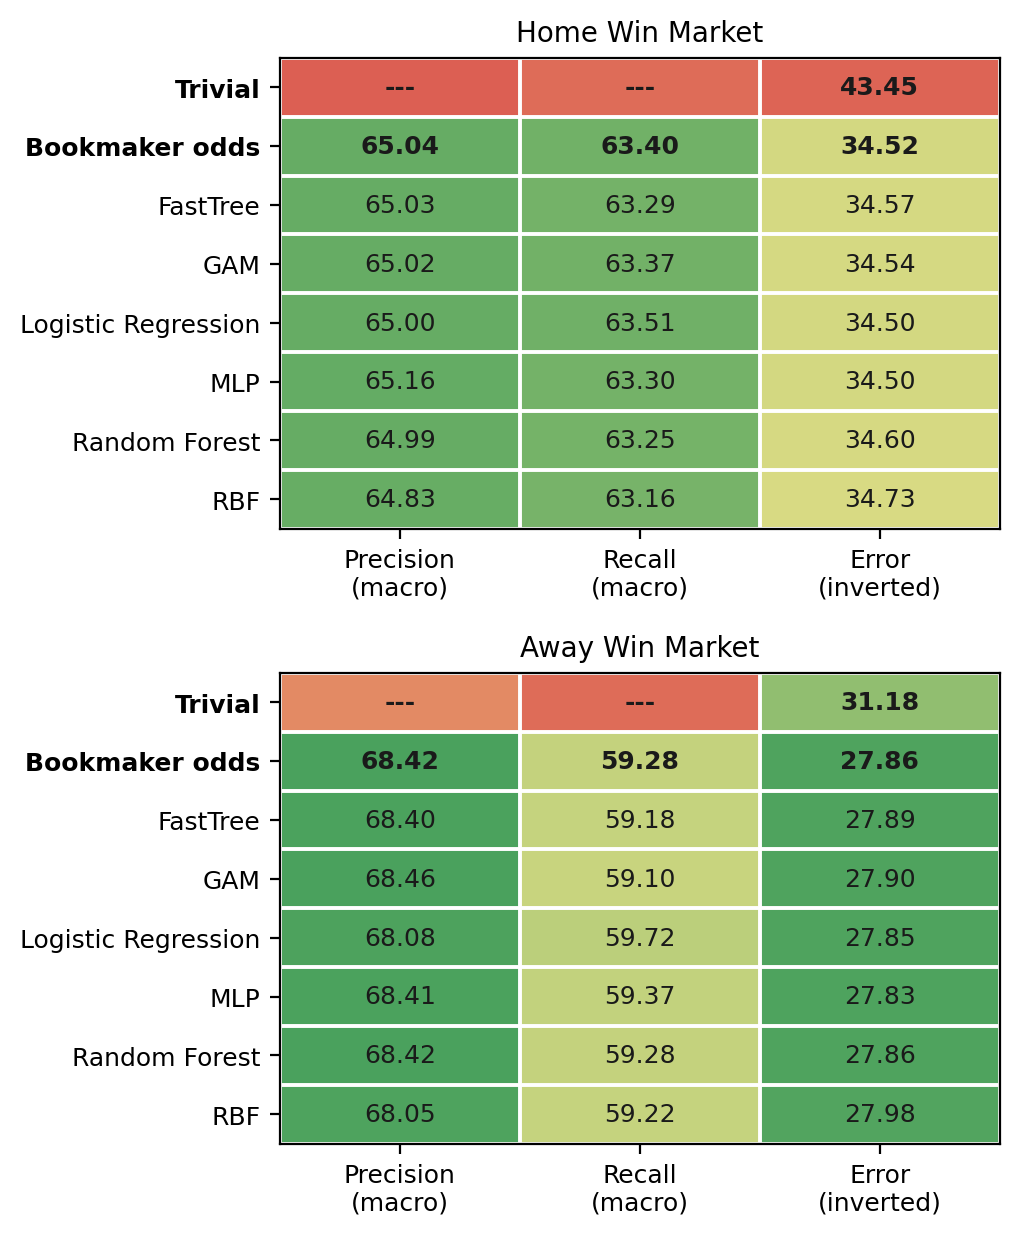
\includegraphics[width=0.95\columnwidth]{all}
\par\end{raggedright}
\caption{Macro-averaged Precision, Recall and Error (\%) for the six classifiers
and the two reference predictors, on the Home Win (top) and Away Win
(bottom) markets. The colour scale is absolute and identical for both
markets, so that differences of a few tenths of a point between models
appear as differences of a few tenths. The Error column is coloured
inverted (100 - Error) so that green denotes better performance throughout;
the numeric labels give the actual values.\label{fig:Heatmap-of-Precision.}}

\end{figure}
The heatmap condenses the results of the two binary markets into a
single panel. Its main message is the uniformity of the colouring:
the six classifiers occupy a narrow band in every column, and no row
is systematically greener than the others.

Five of the six classifiers are stochastic given fixed training data,
so the values reported in the tables above depend to some extent on
the random seed. Table \ref{tab:seed-stability} quantifies that dependence
over 30 refits of each stochastic classifier; logistic regression
was refitted twice, to confirm that it is deterministic. The standard
deviation of the error lies between 0.012 and 0.066 percentage points,
which is small in absolute terms but not negligible relative to the
differences between classifiers: the means themselves span 0.146 percentage
points in the Home Win market, so seed variation does not by itself
account for the ordering of the classifiers. What it does account
for is the distance to the market. In the Home Win market the error
of the de-vigged bookmaker forecast falls inside the range of the
30 refits for four of the six classifiers, and in the Away Win market
for five of the six, while 14 of the 15 pairs of classifiers have
overlapping ranges in the Home Win market and 13 of 15 in the Away
Win market. The observed gap between neighbouring classifiers is therefore
of the same order as the variation induced by the seed alone, and
should not be over-interpreted. The values printed in the results
tables were produced with a single fixed seed, and they fall within
or immediately adjacent to the ranges reported here.

\begin{table}[H]
\caption{Sensitivity of the reported error to the random seed. Each stochastic
classifier was refitted 30 times on the full training set with a different
seed and evaluated on the test set; the table gives the mean error,
its standard deviation and the range observed across those fits. Logistic
regression is deterministic given fixed training data and was refitted
twice to confirm it. The reference row is repeated from the preceding
tables and does not depend on training.\label{tab:seed-stability}}

\centering{}%
\begin{tabular}{ccccc}
\hline 
{\footnotesize\textbf{MODEL}} & \begin{cellvarwidth}[t]
\centering
{\footnotesize\textbf{HOME WIN}}\\
{\footnotesize\textbf{MEAN ERROR}}
\end{cellvarwidth} & \begin{cellvarwidth}[t]
\centering
{\footnotesize\textbf{HOME WIN}}\\
{\footnotesize\textbf{SD {[}MIN, MAX{]}}}
\end{cellvarwidth} & \begin{cellvarwidth}[t]
\centering
{\footnotesize\textbf{AWAY WIN}}\\
{\footnotesize\textbf{MEAN ERROR}}
\end{cellvarwidth} & \begin{cellvarwidth}[t]
\centering
{\footnotesize\textbf{AWAY WIN}}\\
{\footnotesize\textbf{SD {[}MIN, MAX{]}}}
\end{cellvarwidth}\tabularnewline
\hline 
\begin{cellvarwidth}[t]
\centering
{\footnotesize\textbf{Bookmaker odds}}\\
{\footnotesize\textbf{(de-vigged)}}
\end{cellvarwidth} & {\footnotesize\textbf{34.52\%}} & {\footnotesize\textbf{-}} & {\footnotesize\textbf{27.86\%}} & {\footnotesize\textbf{-}}\tabularnewline
{\footnotesize FastTree} & {\footnotesize 34.577\%} & \begin{cellvarwidth}[t]
\centering
{\footnotesize 0.044}\\
{\footnotesize{[}34.487, 34.680{]}}
\end{cellvarwidth} & {\footnotesize 27.884\%} & \begin{cellvarwidth}[t]
\centering
{\footnotesize 0.025}\\
{\footnotesize{[}27.834, 27.936{]}}
\end{cellvarwidth}\tabularnewline
{\footnotesize GAM} & {\footnotesize 34.507\%} & \begin{cellvarwidth}[t]
\centering
{\footnotesize 0.027}\\
{\footnotesize{[}34.457, 34.597{]}}
\end{cellvarwidth} & {\footnotesize 27.875\%} & \begin{cellvarwidth}[t]
\centering
{\footnotesize 0.012}\\
{\footnotesize{[}27.850, 27.892{]}}
\end{cellvarwidth}\tabularnewline
{\footnotesize LogReg} & {\footnotesize 34.500\%} & \begin{cellvarwidth}[t]
\centering
{\footnotesize 0}\\
{\footnotesize{[}34.500, 34.500{]}}
\end{cellvarwidth} & {\footnotesize 27.847\%} & \begin{cellvarwidth}[t]
\centering
{\footnotesize 0}\\
{\footnotesize{[}27.847, 27.847{]}}
\end{cellvarwidth}\tabularnewline
{\footnotesize MLP} & {\footnotesize 34.602\%} & \begin{cellvarwidth}[t]
\centering
{\footnotesize 0.054}\\
{\footnotesize{[}34.490, 34.678{]}}
\end{cellvarwidth} & {\footnotesize 27.899\%} & \begin{cellvarwidth}[t]
\centering
{\footnotesize 0.061}\\
{\footnotesize{[}27.816, 28.087{]}}
\end{cellvarwidth}\tabularnewline
{\footnotesize RF} & {\footnotesize 34.590\%} & \begin{cellvarwidth}[t]
\centering
{\footnotesize 0.029}\\
{\footnotesize{[}34.548, 34.687{]}}
\end{cellvarwidth} & {\footnotesize 27.842\%} & \begin{cellvarwidth}[t]
\centering
{\footnotesize 0.017}\\
{\footnotesize{[}27.814, 27.884{]}}
\end{cellvarwidth}\tabularnewline
{\footnotesize RBF} & {\footnotesize 34.646\%} & \begin{cellvarwidth}[t]
\centering
{\footnotesize 0.066}\\
{\footnotesize{[}34.475, 34.757{]}}
\end{cellvarwidth} & {\footnotesize 27.963\%} & \begin{cellvarwidth}[t]
\centering
{\footnotesize 0.051}\\
{\footnotesize{[}27.855, 28.085{]}}
\end{cellvarwidth}\tabularnewline
\hline 
\end{tabular}
\end{table}

The results tables report the three quantities on which the comparison
with the market turns. For completeness, Tables \ref{tab:full-metrics-home}
and \ref{tab:full-metrics-away} give five further metrics for both
binary markets, each with its 95\% bootstrap CIs: the two threshold-free
measures of ranking quality, the F1 score of the positive class, and
the Brier score and logarithmic loss. The pattern is the one already
described. Every interval for every model overlaps the corresponding
value for the de-vigged market forecast on the probabilistic scores,
and no model attains a higher AUC or average precision than the market
in either market.

For completeness, Table \ref{tab:Draw-experimental} reports the same
binary decomposition applied to the draw outcome. The result is instructive:
for four of the six classifiers, and for the market itself, the precision
and recall of the positive class at the 0.5 threshold are both exactly
zero, because no positive prediction is ever issued; the macro averages
printed in the table are correspondingly the values obtained when
only the negative class is predicted, because the estimated draw probability
almost never exceeds one half. The two classifiers that do issue positive
predictions obtain a high macro precision from very few of them: 62
positive predictions for the MLP and 122 for logistic regression,
out of 75,495 matches, which is why their precision column appears
favourable while their recall of actual draws remains below 0.4 per
cent. Threshold-based measures are therefore uninformative for this
outcome, which motivates the proper scoring rules reported in the
following subsection.

\begin{table}[H]
\caption{Additional metrics for the Home Win market, with 95\% bootstrap CIs.
The three quantities reported in the corresponding results table above
are not repeated here. Precision and recall for the positive class
are summarised by the F1 column; their macro-averaged counterparts
are in Table \ref{tab:Home-win-experimental}. Intervals are percentile
intervals over 1000 resamples of the test set, computed from the same
resamples for every predictor so that the comparisons are paired.\label{tab:full-metrics-home}}

\centering{}%
\begin{tabular}{cccccc}
\hline 
{\footnotesize\textbf{PREDICTOR}} &  & \begin{cellvarwidth}[t]
\centering
{\footnotesize\textbf{AVERAGE}}\\
{\footnotesize\textbf{PRECISION}}
\end{cellvarwidth} & \begin{cellvarwidth}[t]
\centering
{\footnotesize\textbf{F1}}\\
{\footnotesize\textbf{(POSITIVE)}}
\end{cellvarwidth} & {\footnotesize\textbf{BRIER}} & \begin{cellvarwidth}[t]
\centering
{\footnotesize\textbf{LOG}}\\
{\footnotesize\textbf{LOSS}}
\end{cellvarwidth}\tabularnewline
\hline 
\begin{cellvarwidth}[t]
\centering
{\footnotesize\textbf{Bookmaker odds}}\\
{\footnotesize\textbf{(de-vigged)}}
\end{cellvarwidth} & {\footnotesize\textbf{0.7052}} & {\footnotesize\textbf{0.6486}} & {\footnotesize\textbf{54.47\%}} & {\footnotesize\textbf{0.2137}} & {\footnotesize\textbf{0.6149}}\tabularnewline
{\footnotesize FastTree} & \begin{cellvarwidth}[t]
\centering
{\footnotesize 0.7047}\\
{\footnotesize{[}0.7012, 0.7085{]}}
\end{cellvarwidth} & \begin{cellvarwidth}[t]
\centering
{\footnotesize 0.6478}\\
{\footnotesize{[}0.6427, 0.6535{]}}
\end{cellvarwidth} & \begin{cellvarwidth}[t]
\centering
{\footnotesize 54.14\%}\\
{\footnotesize{[}53.64, 54.64{]}}
\end{cellvarwidth} & \begin{cellvarwidth}[t]
\centering
{\footnotesize 0.2139}\\
{\footnotesize{[}0.2128, 0.2150{]}}
\end{cellvarwidth} & \begin{cellvarwidth}[t]
\centering
{\footnotesize 0.6154}\\
{\footnotesize{[}0.6129, 0.6178{]}}
\end{cellvarwidth}\tabularnewline
{\footnotesize GAM} & \begin{cellvarwidth}[t]
\centering
{\footnotesize 0.7050}\\
{\footnotesize{[}0.7013, 0.7087{]}}
\end{cellvarwidth} & \begin{cellvarwidth}[t]
\centering
{\footnotesize 0.6482}\\
{\footnotesize{[}0.6431, 0.6540{]}}
\end{cellvarwidth} & \begin{cellvarwidth}[t]
\centering
{\footnotesize 54.42\%}\\
{\footnotesize{[}53.93, 54.92{]}}
\end{cellvarwidth} & \begin{cellvarwidth}[t]
\centering
{\footnotesize 0.2139}\\
{\footnotesize{[}0.2128, 0.2150{]}}
\end{cellvarwidth} & \begin{cellvarwidth}[t]
\centering
{\footnotesize 0.6153}\\
{\footnotesize{[}0.6129, 0.6178{]}}
\end{cellvarwidth}\tabularnewline
{\footnotesize LogReg} & \begin{cellvarwidth}[t]
\centering
{\footnotesize 0.7051}\\
{\footnotesize{[}0.7015, 0.7089{]}}
\end{cellvarwidth} & \begin{cellvarwidth}[t]
\centering
{\footnotesize 0.6485}\\
{\footnotesize{[}0.6434, 0.6542{]}}
\end{cellvarwidth} & \begin{cellvarwidth}[t]
\centering
{\footnotesize 54.89\%}\\
{\footnotesize{[}54.42, 55.39{]}}
\end{cellvarwidth} & \begin{cellvarwidth}[t]
\centering
{\footnotesize 0.2138}\\
{\footnotesize{[}0.2127, 0.2150{]}}
\end{cellvarwidth} & \begin{cellvarwidth}[t]
\centering
{\footnotesize 0.6154}\\
{\footnotesize{[}0.6129, 0.6179{]}}
\end{cellvarwidth}\tabularnewline
{\footnotesize MLP} & \begin{cellvarwidth}[t]
\centering
{\footnotesize 0.7030}\\
{\footnotesize{[}0.6994, 0.7068{]}}
\end{cellvarwidth} & \begin{cellvarwidth}[t]
\centering
{\footnotesize 0.6462}\\
{\footnotesize{[}0.6409, 0.6519{]}}
\end{cellvarwidth} & \begin{cellvarwidth}[t]
\centering
{\footnotesize 53.94\%}\\
{\footnotesize{[}53.43, 54.46{]}}
\end{cellvarwidth} & \begin{cellvarwidth}[t]
\centering
{\footnotesize 0.2143}\\
{\footnotesize{[}0.2132, 0.2155{]}}
\end{cellvarwidth} & \begin{cellvarwidth}[t]
\centering
{\footnotesize 0.6163}\\
{\footnotesize{[}0.6138, 0.6189{]}}
\end{cellvarwidth}\tabularnewline
{\footnotesize RF} & \begin{cellvarwidth}[t]
\centering
{\footnotesize 0.7044}\\
{\footnotesize{[}0.7009, 0.7081{]}}
\end{cellvarwidth} & \begin{cellvarwidth}[t]
\centering
{\footnotesize 0.6477}\\
{\footnotesize{[}0.6426, 0.6534{]}}
\end{cellvarwidth} & \begin{cellvarwidth}[t]
\centering
{\footnotesize 54.06\%}\\
{\footnotesize{[}53.57, 54.55{]}}
\end{cellvarwidth} & \begin{cellvarwidth}[t]
\centering
{\footnotesize 0.2140}\\
{\footnotesize{[}0.2129, 0.2151{]}}
\end{cellvarwidth} & \begin{cellvarwidth}[t]
\centering
{\footnotesize 0.6154}\\
{\footnotesize{[}0.6129, 0.6179{]}}
\end{cellvarwidth}\tabularnewline
{\footnotesize RBF} & \begin{cellvarwidth}[t]
\centering
{\footnotesize 0.7023}\\
{\footnotesize{[}0.6989, 0.7060{]}}
\end{cellvarwidth} & \begin{cellvarwidth}[t]
\centering
{\footnotesize 0.6442}\\
{\footnotesize{[}0.6390, 0.6498{]}}
\end{cellvarwidth} & \begin{cellvarwidth}[t]
\centering
{\footnotesize 54.04\%}\\
{\footnotesize{[}53.57, 54.55{]}}
\end{cellvarwidth} & \begin{cellvarwidth}[t]
\centering
{\footnotesize 0.2146}\\
{\footnotesize{[}0.2134, 0.2156{]}}
\end{cellvarwidth} & \begin{cellvarwidth}[t]
\centering
{\footnotesize 0.6170}\\
{\footnotesize{[}0.6144, 0.6194{]}}
\end{cellvarwidth}\tabularnewline
\hline 
\end{tabular}
\end{table}

\begin{table}[H]
\caption{Additional metrics for the Away Win market, with 95\% bootstrap CIs.
The three quantities reported in the corresponding results table above
are not repeated here. Precision and recall for the positive class
are summarised by the F1 column; their macro-averaged counterparts
are in Table \ref{tab:Away-win-experimental}. Intervals are percentile
intervals over 1000 resamples of the test set, computed from the same
resamples for every predictor so that the comparisons are paired.\label{tab:full-metrics-away}}

\centering{}%
\begin{tabular}{cccccc}
\hline 
{\footnotesize\textbf{PREDICTOR}} &  & \begin{cellvarwidth}[t]
\centering
{\footnotesize\textbf{AVERAGE}}\\
{\footnotesize\textbf{PRECISION}}
\end{cellvarwidth} & \begin{cellvarwidth}[t]
\centering
{\footnotesize\textbf{F1}}\\
{\footnotesize\textbf{(POSITIVE)}}
\end{cellvarwidth} & {\footnotesize\textbf{BRIER}} & \begin{cellvarwidth}[t]
\centering
{\footnotesize\textbf{LOG}}\\
{\footnotesize\textbf{LOSS}}
\end{cellvarwidth}\tabularnewline
\hline 
\begin{cellvarwidth}[t]
\centering
{\footnotesize\textbf{Bookmaker odds}}\\
{\footnotesize\textbf{(de-vigged)}}
\end{cellvarwidth} & {\footnotesize\textbf{0.7139}} & {\footnotesize\textbf{0.5416}} & {\footnotesize\textbf{35.98\%}} & {\footnotesize\textbf{0.1868}} & {\footnotesize\textbf{0.5538}}\tabularnewline
{\footnotesize FastTree} & \begin{cellvarwidth}[t]
\centering
{\footnotesize 0.7129}\\
{\footnotesize{[}0.7091, 0.7169{]}}
\end{cellvarwidth} & \begin{cellvarwidth}[t]
\centering
{\footnotesize 0.5398}\\
{\footnotesize{[}0.5331, 0.5472{]}}
\end{cellvarwidth} & \begin{cellvarwidth}[t]
\centering
{\footnotesize 35.70\%}\\
{\footnotesize{[}35.07, 36.43{]}}
\end{cellvarwidth} & \begin{cellvarwidth}[t]
\centering
{\footnotesize 0.1871}\\
{\footnotesize{[}0.1858, 0.1885{]}}
\end{cellvarwidth} & \begin{cellvarwidth}[t]
\centering
{\footnotesize 0.5546}\\
{\footnotesize{[}0.5514, 0.5578{]}}
\end{cellvarwidth}\tabularnewline
{\footnotesize GAM} & \begin{cellvarwidth}[t]
\centering
{\footnotesize 0.7136}\\
{\footnotesize{[}0.7097, 0.7176{]}}
\end{cellvarwidth} & \begin{cellvarwidth}[t]
\centering
{\footnotesize 0.5409}\\
{\footnotesize{[}0.5343, 0.5479{]}}
\end{cellvarwidth} & \begin{cellvarwidth}[t]
\centering
{\footnotesize 35.43\%}\\
{\footnotesize{[}34.80, 36.15{]}}
\end{cellvarwidth} & \begin{cellvarwidth}[t]
\centering
{\footnotesize 0.1870}\\
{\footnotesize{[}0.1856, 0.1884{]}}
\end{cellvarwidth} & \begin{cellvarwidth}[t]
\centering
{\footnotesize 0.5543}\\
{\footnotesize{[}0.5510, 0.5575{]}}
\end{cellvarwidth}\tabularnewline
{\footnotesize LogReg} & \begin{cellvarwidth}[t]
\centering
{\footnotesize 0.7133}\\
{\footnotesize{[}0.7094, 0.7173{]}}
\end{cellvarwidth} & \begin{cellvarwidth}[t]
\centering
{\footnotesize 0.5409}\\
{\footnotesize{[}0.5344, 0.5480{]}}
\end{cellvarwidth} & \begin{cellvarwidth}[t]
\centering
{\footnotesize 37.41\%}\\
{\footnotesize{[}36.81, 38.12{]}}
\end{cellvarwidth} & \begin{cellvarwidth}[t]
\centering
{\footnotesize 0.1871}\\
{\footnotesize{[}0.1857, 0.1885{]}}
\end{cellvarwidth} & \begin{cellvarwidth}[t]
\centering
{\footnotesize 0.5548}\\
{\footnotesize{[}0.5515, 0.5580{]}}
\end{cellvarwidth}\tabularnewline
{\footnotesize MLP} & \begin{cellvarwidth}[t]
\centering
{\footnotesize 0.7128}\\
{\footnotesize{[}0.7089, 0.7170{]}}
\end{cellvarwidth} & \begin{cellvarwidth}[t]
\centering
{\footnotesize 0.5395}\\
{\footnotesize{[}0.5329, 0.5466{]}}
\end{cellvarwidth} & \begin{cellvarwidth}[t]
\centering
{\footnotesize 36.26\%}\\
{\footnotesize{[}35.63, 36.93{]}}
\end{cellvarwidth} & \begin{cellvarwidth}[t]
\centering
{\footnotesize 0.1872}\\
{\footnotesize{[}0.1857, 0.1886{]}}
\end{cellvarwidth} & \begin{cellvarwidth}[t]
\centering
{\footnotesize 0.5545}\\
{\footnotesize{[}0.5512, 0.5579{]}}
\end{cellvarwidth}\tabularnewline
{\footnotesize RF} & \begin{cellvarwidth}[t]
\centering
{\footnotesize 0.7133}\\
{\footnotesize{[}0.7095, 0.7174{]}}
\end{cellvarwidth} & \begin{cellvarwidth}[t]
\centering
{\footnotesize 0.5402}\\
{\footnotesize{[}0.5336, 0.5472{]}}
\end{cellvarwidth} & \begin{cellvarwidth}[t]
\centering
{\footnotesize 35.98\%}\\
{\footnotesize{[}35.33, 36.70{]}}
\end{cellvarwidth} & \begin{cellvarwidth}[t]
\centering
{\footnotesize 0.1871}\\
{\footnotesize{[}0.1857, 0.1885{]}}
\end{cellvarwidth} & \begin{cellvarwidth}[t]
\centering
{\footnotesize 0.5544}\\
{\footnotesize{[}0.5512, 0.5576{]}}
\end{cellvarwidth}\tabularnewline
{\footnotesize RBF} & \begin{cellvarwidth}[t]
\centering
{\footnotesize 0.7108}\\
{\footnotesize{[}0.7068, 0.7149{]}}
\end{cellvarwidth} & \begin{cellvarwidth}[t]
\centering
{\footnotesize 0.5360}\\
{\footnotesize{[}0.5290, 0.5428{]}}
\end{cellvarwidth} & \begin{cellvarwidth}[t]
\centering
{\footnotesize 35.98\%}\\
{\footnotesize{[}35.34, 36.67{]}}
\end{cellvarwidth} & \begin{cellvarwidth}[t]
\centering
{\footnotesize 0.1878}\\
{\footnotesize{[}0.1864, 0.1892{]}}
\end{cellvarwidth} & \begin{cellvarwidth}[t]
\centering
{\footnotesize 0.5562}\\
{\footnotesize{[}0.5530, 0.5594{]}}
\end{cellvarwidth}\tabularnewline
\hline 
\end{tabular}
\end{table}

\begin{table}[H]
\caption{Draw market experimental results. Precision and recall are macro averages
across both classes. Each model cell gives the point estimate and,
beneath it, the 95\% bootstrap CI over 1000 paired resamples of the
test set. The two reference predictors are computed without training
and are reported as point estimates.\label{tab:Draw-experimental}}

\centering{}%
\begin{tabular}{cccc}
\hline 
\textbf{MODEL} & \textbf{ERROR} & \begin{cellvarwidth}[t]
\centering
\textbf{PRECISION}\\
\textbf{(macro)}
\end{cellvarwidth} & \begin{cellvarwidth}[t]
\centering
\textbf{RECALL}\\
\textbf{(macro)}
\end{cellvarwidth}\tabularnewline
\hline 
\begin{cellvarwidth}[t]
\centering
\textbf{Trivial}\\
\textbf{(majority class)}
\end{cellvarwidth} & \textbf{25.37\%} & \textbf{-} & \textbf{-}\tabularnewline
\begin{cellvarwidth}[t]
\centering
\textbf{Bookmaker odds}\\
\textbf{(de-vigged)}
\end{cellvarwidth} & \textbf{25.37\%} & \textbf{37.32\%} & \textbf{50.00\%}\tabularnewline
FastTree & \begin{cellvarwidth}[t]
\centering
25.37\%\\
{[}25.05, 25.69{]}
\end{cellvarwidth} & \begin{cellvarwidth}[t]
\centering
37.32\%\\
{[}37.16, 37.47{]}
\end{cellvarwidth} & \begin{cellvarwidth}[t]
\centering
50.00\%\\
{[}50.00, 50.00{]}
\end{cellvarwidth}\tabularnewline
GAM & \begin{cellvarwidth}[t]
\centering
25.37\%\\
{[}25.05, 25.69{]}
\end{cellvarwidth} & \begin{cellvarwidth}[t]
\centering
37.32\%\\
{[}37.16, 37.47{]}
\end{cellvarwidth} & \begin{cellvarwidth}[t]
\centering
50.00\%\\
{[}50.00, 50.00{]}
\end{cellvarwidth}\tabularnewline
LogReg & \begin{cellvarwidth}[t]
\centering
25.36\%\\
{[}25.03, 25.67{]}
\end{cellvarwidth} & \begin{cellvarwidth}[t]
\centering
63.98\%\\
{[}59.51, 68.50{]}
\end{cellvarwidth} & \begin{cellvarwidth}[t]
\centering
50.12\%\\
{[}50.08, 50.17{]}
\end{cellvarwidth}\tabularnewline
MLP & \begin{cellvarwidth}[t]
\centering
25.33\%\\
{[}25.01, 25.65{]}
\end{cellvarwidth} & \begin{cellvarwidth}[t]
\centering
74.43\%\\
{[}68.64, 80.01{]}
\end{cellvarwidth} & \begin{cellvarwidth}[t]
\centering
50.11\%\\
{[}50.07, 50.14{]}
\end{cellvarwidth}\tabularnewline
RF & \begin{cellvarwidth}[t]
\centering
25.37\%\\
{[}25.05, 25.69{]}
\end{cellvarwidth} & \begin{cellvarwidth}[t]
\centering
37.32\%\\
{[}37.16, 37.47{]}
\end{cellvarwidth} & \begin{cellvarwidth}[t]
\centering
50.00\%\\
{[}50.00, 50.00{]}
\end{cellvarwidth}\tabularnewline
RBF & \begin{cellvarwidth}[t]
\centering
25.37\%\\
{[}25.05, 25.69{]}
\end{cellvarwidth} & \begin{cellvarwidth}[t]
\centering
37.32\%\\
{[}37.16, 37.47{]}
\end{cellvarwidth} & \begin{cellvarwidth}[t]
\centering
50.00\%\\
{[}50.00, 50.00{]}
\end{cellvarwidth}\tabularnewline
\hline 
\end{tabular}
\end{table}


\subsection{Three-class classification results}

The binary formulation above merges two of the three outcomes into
a single negative class. For completeness, this subsection reports
the three-class problem (home win, draw, away win) as a single multinomial
classification task. This formulation has the additional property
that the predicted probabilities sum to one by construction, which
makes them directly comparable with the de-vigged market probabilities.
Because no natural decision threshold exists in the three-class setting,
performance is reported using accuracy together with three threshold-free
scoring rules \citep{gneiting2007,constantinou2012}: multiclass logarithmic
loss, the multiclass Brier score, and the RPS, which exploits the
ordering of the outcome and penalises errors between adjacent categories
less heavily than errors between extremes. Its suitability for football
forecasts has been questioned \citep{wheatcroft2021}, and it is therefore
reported alongside the logarithmic loss and the Brier score rather
than on its own. All values are accompanied by 95\% bootstrap CIs
obtained from 1000 paired resamples of the test set \citep{efron1993}.

Two reference predictors are included in both tables. The trivial
predictor assigns the class frequencies observed in the training set
to every match. The bookmaker predictor is the de-vigged market probability
itself, evaluated as a classifier without any training. Table \ref{tab:three-class-no-odds}
reports the results obtained when the market probabilities are excluded
from the feature set, and Table \ref{tab:three-class-with-odds} the
results obtained when they are included.

\begin{table}[H]
\caption{Three-class classification without odds-based features. Each cell
gives the point estimate followed by the 95\% bootstrap CIs in brackets
(1000 paired resamples of the test set). Higher accuracy is better;
lower LogLoss, Brier and RPS are better.\label{tab:three-class-no-odds}}

{\footnotesize{}%
\begin{tabular}{>{\centering}p{2.6cm}>{\centering}p{2.28cm}>{\centering}p{2.28cm}>{\centering}p{2.28cm}>{\centering}p{2.28cm}}
\hline 
{\footnotesize\textbf{PREDICTOR}} & {\footnotesize\textbf{ACCURACY (\%)}} & {\footnotesize\textbf{LOGLOSS}} & {\footnotesize\textbf{BRIER}} & {\footnotesize\textbf{RPS}}\tabularnewline
\hline 
{\footnotesize\textbf{Trivial}} & {\footnotesize\textbf{43.45}}\\
{\footnotesize\textbf{{[}43.10, 43.81{]}}} & {\footnotesize\textbf{1.0738}}\\
{\footnotesize\textbf{{[}1.0721, 1.0755{]}}} & {\footnotesize\textbf{0.6498}}\\
{\footnotesize\textbf{{[}0.6486, 0.6509{]}}} & {\footnotesize\textbf{0.2302}}\\
{\footnotesize\textbf{{[}0.2298, 0.2307{]}}}\tabularnewline
{\footnotesize\textbf{Bookmaker odds}} & {\footnotesize\textbf{51.89}}\\
{\footnotesize\textbf{{[}51.53, 52.27{]}}} & {\footnotesize\textbf{0.9836}}\\
{\footnotesize\textbf{{[}0.9803, 0.9867{]}}} & {\footnotesize\textbf{0.5865}}\\
{\footnotesize\textbf{{[}0.5841, 0.5887{]}}} & {\footnotesize\textbf{0.2003}}\\
{\footnotesize\textbf{{[}0.1994, 0.2012{]}}}\tabularnewline
{\footnotesize FastTree} & {\footnotesize 48.01}\\
{\footnotesize{[}47.66, 48.37{]}} & {\footnotesize 1.0301}\\
{\footnotesize{[}1.0273, 1.0328{]}} & {\footnotesize 0.6183}\\
{\footnotesize{[}0.6163, 0.6202{]}} & {\footnotesize 0.2149}\\
{\footnotesize{[}0.2141, 0.2157{]}}\tabularnewline
{\footnotesize GAM} & {\footnotesize 48.00}\\
{\footnotesize{[}47.65, 48.37{]}} & {\footnotesize 1.0293}\\
{\footnotesize{[}1.0266, 1.0320{]}} & {\footnotesize 0.6178}\\
{\footnotesize{[}0.6159, 0.6198{]}} & {\footnotesize 0.2148}\\
{\footnotesize{[}0.2140, 0.2156{]}}\tabularnewline
{\footnotesize LogReg} & {\footnotesize 48.02}\\
{\footnotesize{[}47.67, 48.38{]}} & {\footnotesize 1.0289}\\
{\footnotesize{[}1.0262, 1.0318{]}} & {\footnotesize 0.6176}\\
{\footnotesize{[}0.6157, 0.6196{]}} & {\footnotesize 0.2147}\\
{\footnotesize{[}0.2139, 0.2155{]}}\tabularnewline
{\footnotesize RF} & {\footnotesize 48.04}\\
{\footnotesize{[}47.68, 48.40{]}} & {\footnotesize 1.0296}\\
{\footnotesize{[}1.0269, 1.0324{]}} & {\footnotesize 0.6180}\\
{\footnotesize{[}0.6161, 0.6200{]}} & {\footnotesize 0.2148}\\
{\footnotesize{[}0.2140, 0.2156{]}}\tabularnewline
{\footnotesize MLP} & {\footnotesize 47.96}\\
{\footnotesize{[}47.62, 48.33{]}} & {\footnotesize 1.0302}\\
{\footnotesize{[}1.0275, 1.0330{]}} & {\footnotesize 0.6185}\\
{\footnotesize{[}0.6165, 0.6204{]}} & {\footnotesize 0.2150}\\
{\footnotesize{[}0.2143, 0.2158{]}}\tabularnewline
{\footnotesize RBF} & {\footnotesize 48.01}\\
{\footnotesize{[}47.67, 48.37{]}} & {\footnotesize 1.0301}\\
{\footnotesize{[}1.0272, 1.0330{]}} & {\footnotesize 0.6183}\\
{\footnotesize{[}0.6163, 0.6204{]}} & {\footnotesize 0.2150}\\
{\footnotesize{[}0.2142, 0.2158{]}}\tabularnewline
\hline 
\end{tabular}}{\footnotesize\par}
\end{table}

Without odds-based features, all six classifiers fall within 0.08
accuracy points of one another (47.96-48.04\%), while the distance
between the trivial baseline and the market is 8.4 points. This indicates
that the limiting factor is the information available in the feature
set rather than the choice of learning algorithm. The models nevertheless
recover approximately half of that gap, improving on the trivial baseline
by 4.6 accuracy points and by approximately 0.045 in logarithmic loss.

\begin{table}[H]
\caption{Three-class classification with odds-based features included. Each
cell gives the point estimate followed by the 95\% bootstrap CI in
brackets (1000 paired resamples of the test set).\label{tab:three-class-with-odds}}

{\footnotesize{}%
\begin{tabular}{>{\centering}p{2.6cm}>{\centering}p{2.28cm}>{\centering}p{2.28cm}>{\centering}p{2.28cm}>{\centering}p{2.28cm}}
\hline 
{\footnotesize\textbf{PREDICTOR}} & {\footnotesize\textbf{ACCURACY (\%)}} & {\footnotesize\textbf{LOGLOSS}} & {\footnotesize\textbf{BRIER}} & {\footnotesize\textbf{RPS}}\tabularnewline
\hline 
{\footnotesize\textbf{Trivial}} & {\footnotesize\textbf{43.45}}\\
{\footnotesize\textbf{{[}43.10, 43.81{]}}} & {\footnotesize\textbf{1.0738}}\\
{\footnotesize\textbf{{[}1.0721, 1.0755{]}}} & {\footnotesize\textbf{0.6498}}\\
{\footnotesize\textbf{{[}0.6486, 0.6509{]}}} & {\footnotesize\textbf{0.2302}}\\
{\footnotesize\textbf{{[}0.2298, 0.2307{]}}}\tabularnewline
{\footnotesize\textbf{Bookmaker odds}} & {\footnotesize\textbf{51.89}}\\
{\footnotesize\textbf{{[}51.53, 52.27{]}}} & {\footnotesize\textbf{0.9836}}\\
{\footnotesize\textbf{{[}0.9803, 0.9867{]}}} & {\footnotesize\textbf{0.5865}}\\
{\footnotesize\textbf{{[}0.5841, 0.5887{]}}} & {\footnotesize\textbf{0.2003}}\\
{\footnotesize\textbf{{[}0.1994, 0.2012{]}}}\tabularnewline
{\footnotesize FastTree} & {\footnotesize 51.92}\\
{\footnotesize{[}51.56, 52.27{]}} & {\footnotesize 0.9849}\\
{\footnotesize{[}0.9817, 0.9881{]}} & {\footnotesize 0.5872}\\
{\footnotesize{[}0.5849, 0.5895{]}} & {\footnotesize 0.2006}\\
{\footnotesize{[}0.1997, 0.2014{]}}\tabularnewline
{\footnotesize GAM} & {\footnotesize 51.97}\\
{\footnotesize{[}51.62, 52.35{]}} & {\footnotesize 0.9843}\\
{\footnotesize{[}0.9811, 0.9874{]}} & {\footnotesize 0.5868}\\
{\footnotesize{[}0.5845, 0.5890{]}} & {\footnotesize 0.2004}\\
{\footnotesize{[}0.1995, 0.2013{]}}\tabularnewline
{\footnotesize LogReg} & {\footnotesize 51.87}\\
{\footnotesize{[}51.50, 52.22{]}} & {\footnotesize 0.9845}\\
{\footnotesize{[}0.9812, 0.9877{]}} & {\footnotesize 0.5868}\\
{\footnotesize{[}0.5844, 0.5890{]}} & {\footnotesize 0.2004}\\
{\footnotesize{[}0.1995, 0.2013{]}}\tabularnewline
{\footnotesize RF} & {\footnotesize 51.88}\\
{\footnotesize{[}51.51, 52.24{]}} & {\footnotesize 0.9846}\\
{\footnotesize{[}0.9813, 0.9878{]}} & {\footnotesize 0.5871}\\
{\footnotesize{[}0.5848, 0.5893{]}} & {\footnotesize 0.2005}\\
{\footnotesize{[}0.1996, 0.2014{]}}\tabularnewline
{\footnotesize MLP} & {\footnotesize 51.86}\\
{\footnotesize{[}51.51, 52.23{]}} & {\footnotesize 0.9848}\\
{\footnotesize{[}0.9816, 0.9879{]}} & {\footnotesize 0.5872}\\
{\footnotesize{[}0.5849, 0.5894{]}} & {\footnotesize 0.2006}\\
{\footnotesize{[}0.1997, 0.2015{]}}\tabularnewline
{\footnotesize RBF} & {\footnotesize 51.70}\\
{\footnotesize{[}51.35, 52.06{]}} & {\footnotesize 0.9873}\\
{\footnotesize{[}0.9840, 0.9905{]}} & {\footnotesize 0.5887}\\
{\footnotesize{[}0.5864, 0.5909{]}} & {\footnotesize 0.2011}\\
{\footnotesize{[}0.2003, 0.2020{]}}\tabularnewline
\hline 
\end{tabular}}{\footnotesize\par}
\end{table}

When the market probabilities are included, every model reproduces
the bookmaker forecast to within 0.2 accuracy points. Paired bootstrap
comparisons \citep{efron1993}\textbf{ give the difference between
each classifier and the market on the same resamples, and are reported
in Table \ref{tab:paired-vs-market}. On the three proper scoring
rules the outcome is not merely an absence of improvement: for every
classifier the difference is positive and its interval lies entirely
above zero, so each is significantly worse than the market on the
logarithmic loss, the Brier score and the RPS. On accuracy, four of
the six classifiers have intervals that contain zero. GAM is the only
classifier with a favourable non-zero difference, +0.086 points (95\%
CI {[}0.005, 0.158{]}), a difference corresponding to approximately
65 additional correct predictions out of 75,495 and not accompanied
by any improvement in the probabilistic scores; RBF also excludes
zero, but in the unfavourable direction, -0.192 points (95\% CI {[}-0.314,
-0.066{]}).}

\begin{table}[H]
\caption{Paired differences between each classifier and the de-vigged bookmaker
forecast in the three-class formulation with market probabilities
among the inputs. Each entry is the classifier minus the market on
the same 1000 paired resamples of the test set, with the 95\% percentile
interval of that difference beneath it. Accuracy is in percentage
points and higher is better; for the logarithmic loss, the Brier score
and the ranked probability score lower is better, so a positive difference
denotes worse performance than the market. The quantities are the
paired counterparts of the values in Table \ref{tab:three-class-with-odds}.\label{tab:paired-vs-market}}

\centering{}%
\begin{tabular}{ccccc}
\hline 
{\footnotesize\textbf{PREDICTOR}} & \begin{cellvarwidth}[t]
\centering
{\footnotesize\textbf{ACCURACY}}\\
{\footnotesize\textbf{(points)}}
\end{cellvarwidth} & \begin{cellvarwidth}[t]
\centering
{\footnotesize\textbf{LOG}}\\
{\footnotesize\textbf{LOSS}}
\end{cellvarwidth} & {\footnotesize\textbf{BRIER}} & {\footnotesize\textbf{RPS}}\tabularnewline
\hline 
{\footnotesize FastTree} & \begin{cellvarwidth}[t]
\centering
{\footnotesize +0.031}\\
{\footnotesize{[}-0.069, +0.129{]}}
\end{cellvarwidth} & \begin{cellvarwidth}[t]
\centering
{\footnotesize +0.0013}\\
{\footnotesize{[}+0.0009, +0.0018{]}}
\end{cellvarwidth} & \begin{cellvarwidth}[t]
\centering
{\footnotesize +0.0008}\\
{\footnotesize{[}+0.0005, +0.0010{]}}
\end{cellvarwidth} & \begin{cellvarwidth}[t]
\centering
{\footnotesize +0.0003}\\
{\footnotesize{[}+0.0002, +0.0004{]}}
\end{cellvarwidth}\tabularnewline
{\footnotesize GAM} & \begin{cellvarwidth}[t]
\centering
{\footnotesize +0.086}\\
{\footnotesize{[}+0.005, +0.158{]}}
\end{cellvarwidth} & \begin{cellvarwidth}[t]
\centering
{\footnotesize +0.0008}\\
{\footnotesize{[}+0.0004, +0.0011{]}}
\end{cellvarwidth} & \begin{cellvarwidth}[t]
\centering
{\footnotesize +0.0004}\\
{\footnotesize{[}+0.0002, +0.0006{]}}
\end{cellvarwidth} & \begin{cellvarwidth}[t]
\centering
{\footnotesize +0.0001}\\
{\footnotesize{[}+0.0001, +0.0002{]}}
\end{cellvarwidth}\tabularnewline
{\footnotesize LogReg} & \begin{cellvarwidth}[t]
\centering
{\footnotesize -0.025}\\
{\footnotesize{[}-0.099, +0.041{]}}
\end{cellvarwidth} & \begin{cellvarwidth}[t]
\centering
{\footnotesize +0.0009}\\
{\footnotesize{[}+0.0006, +0.0013{]}}
\end{cellvarwidth} & \begin{cellvarwidth}[t]
\centering
{\footnotesize +0.0003}\\
{\footnotesize{[}+0.0002, +0.0005{]}}
\end{cellvarwidth} & \begin{cellvarwidth}[t]
\centering
{\footnotesize +0.0001}\\
{\footnotesize{[}+0.0001, +0.0002{]}}
\end{cellvarwidth}\tabularnewline
{\footnotesize RF} & \begin{cellvarwidth}[t]
\centering
{\footnotesize -0.013}\\
{\footnotesize{[}-0.117, +0.105{]}}
\end{cellvarwidth} & \begin{cellvarwidth}[t]
\centering
{\footnotesize +0.0010}\\
{\footnotesize{[}+0.0006, +0.0014{]}}
\end{cellvarwidth} & \begin{cellvarwidth}[t]
\centering
{\footnotesize +0.0006}\\
{\footnotesize{[}+0.0003, +0.0009{]}}
\end{cellvarwidth} & \begin{cellvarwidth}[t]
\centering
{\footnotesize +0.0002}\\
{\footnotesize{[}+0.0001, +0.0003{]}}
\end{cellvarwidth}\tabularnewline
{\footnotesize MLP} & \begin{cellvarwidth}[t]
\centering
{\footnotesize -0.031}\\
{\footnotesize{[}-0.134, +0.074{]}}
\end{cellvarwidth} & \begin{cellvarwidth}[t]
\centering
{\footnotesize +0.0012}\\
{\footnotesize{[}+0.0008, +0.0017{]}}
\end{cellvarwidth} & \begin{cellvarwidth}[t]
\centering
{\footnotesize +0.0008}\\
{\footnotesize{[}+0.0005, +0.0010{]}}
\end{cellvarwidth} & \begin{cellvarwidth}[t]
\centering
{\footnotesize +0.0003}\\
{\footnotesize{[}+0.0002, +0.0004{]}}
\end{cellvarwidth}\tabularnewline
{\footnotesize RBF} & \begin{cellvarwidth}[t]
\centering
{\footnotesize -0.192}\\
{\footnotesize{[}-0.314, -0.066{]}}
\end{cellvarwidth} & \begin{cellvarwidth}[t]
\centering
{\footnotesize +0.0037}\\
{\footnotesize{[}+0.0030, +0.0044{]}}
\end{cellvarwidth} & \begin{cellvarwidth}[t]
\centering
{\footnotesize +0.0022}\\
{\footnotesize{[}+0.0018, +0.0026{]}}
\end{cellvarwidth} & \begin{cellvarwidth}[t]
\centering
{\footnotesize +0.0008}\\
{\footnotesize{[}+0.0007, +0.0010{]}}
\end{cellvarwidth}\tabularnewline
\hline 
\end{tabular}
\end{table}

The behaviour of the predictors on the draw class is worth setting
out directly. Table \ref{tab:predicted-class-distribution} gives
the number of matches assigned to each outcome under the arg-max rule.
Draws make up 25.37\% of the test set, but no predictor assigns them
at anything approaching that rate. Without the odds-based features
three of the six classifiers never predict a draw at all, and the
remaining ones do so between 14 and 15 times out of 75,495. With the
odds included every classifier predicts some draws, between 211 and
728 matches, and the de-vigged market itself predicts 396, that is
0.52\% of fixtures. The draw is therefore almost never the most probable
of the three outcomes, for the market no less than for the models,
and this is a property of the outcome rather than a defect of any
one predictor.

\begin{table}[H]
\caption{Distribution of predicted classes in the three-class formulation.
Each row gives the number of the 75,495 test matches assigned to a
home win (1), a draw (X) and an away win (2) under the arg-max rule,
for the design without and the design with the odds-based features.
The observed row gives the realised frequencies over the same matches;
the two reference predictors do not depend on the model inputs and
their counts are therefore identical in both designs.\label{tab:predicted-class-distribution}}

\centering{}%
\begin{tabular}{ccccccc}
\hline 
{\footnotesize\textbf{PREDICTOR}} & \begin{cellvarwidth}[t]
\centering
{\footnotesize\textbf{WITHOUT}}\\
{\footnotesize\textbf{ODDS: 1}}
\end{cellvarwidth} & \begin{cellvarwidth}[t]
\centering
{\footnotesize\textbf{WITHOUT}}\\
{\footnotesize\textbf{ODDS: X}}
\end{cellvarwidth} & \begin{cellvarwidth}[t]
\centering
{\footnotesize\textbf{WITHOUT}}\\
{\footnotesize\textbf{ODDS: 2}}
\end{cellvarwidth} & \begin{cellvarwidth}[t]
\centering
{\footnotesize\textbf{WITH}}\\
{\footnotesize\textbf{ODDS: 1}}
\end{cellvarwidth} & \begin{cellvarwidth}[t]
\centering
{\footnotesize\textbf{WITH}}\\
{\footnotesize\textbf{ODDS: X}}
\end{cellvarwidth} & \begin{cellvarwidth}[t]
\centering
{\footnotesize\textbf{WITH}}\\
{\footnotesize\textbf{ODDS: 2}}
\end{cellvarwidth}\tabularnewline
\hline 
\begin{cellvarwidth}[t]
\centering
{\footnotesize\textbf{Observed}}\\
{\footnotesize\textbf{(test set)}}
\end{cellvarwidth} & {\footnotesize\textbf{32,801}} & {\footnotesize\textbf{19,152}} & {\footnotesize\textbf{23,542}} & {\footnotesize\textbf{32,801}} & {\footnotesize\textbf{19,152}} & {\footnotesize\textbf{23,542}}\tabularnewline
\begin{cellvarwidth}[t]
\centering
{\footnotesize\textbf{Trivial}}\\
{\footnotesize\textbf{(majority class)}}
\end{cellvarwidth} & {\footnotesize\textbf{75,495}} & {\footnotesize\textbf{0}} & {\footnotesize\textbf{0}} & {\footnotesize\textbf{75,495}} & {\footnotesize\textbf{0}} & {\footnotesize\textbf{0}}\tabularnewline
\begin{cellvarwidth}[t]
\centering
{\footnotesize\textbf{Bookmaker odds}}\\
{\footnotesize\textbf{(de-vigged)}}
\end{cellvarwidth} & {\footnotesize\textbf{50,308}} & {\footnotesize\textbf{396}} & {\footnotesize\textbf{24,791}} & {\footnotesize\textbf{50,308}} & {\footnotesize\textbf{396}} & {\footnotesize\textbf{24,791}}\tabularnewline
{\footnotesize FastTree} & {\footnotesize 52,180} & {\footnotesize 15} & {\footnotesize 23,300} & {\footnotesize 50,499} & {\footnotesize 607} & {\footnotesize 24,389}\tabularnewline
{\footnotesize GAM} & {\footnotesize 51,671} & {\footnotesize 0} & {\footnotesize 23,824} & {\footnotesize 49,740} & {\footnotesize 211} & {\footnotesize 25,544}\tabularnewline
{\footnotesize LogReg} & {\footnotesize 51,116} & {\footnotesize 0} & {\footnotesize 24,379} & {\footnotesize 49,651} & {\footnotesize 728} & {\footnotesize 25,116}\tabularnewline
{\footnotesize MLP} & {\footnotesize 49,974} & {\footnotesize 14} & {\footnotesize 25,507} & {\footnotesize 50,307} & {\footnotesize 631} & {\footnotesize 24,557}\tabularnewline
{\footnotesize RF} & {\footnotesize 51,562} & {\footnotesize 0} & {\footnotesize 23,933} & {\footnotesize 50,732} & {\footnotesize 435} & {\footnotesize 24,328}\tabularnewline
{\footnotesize RBF} & {\footnotesize 52,203} & {\footnotesize 14} & {\footnotesize 23,278} & {\footnotesize 50,087} & {\footnotesize 683} & {\footnotesize 24,725}\tabularnewline
\hline 
\end{tabular}
\end{table}

Because both formulations are estimated on the same features and the
same chronological split, the difference between the numbers they
report arises from the encoding of the outcome and from the evaluation
metric that goes with it, and not from the inputs. The binary tables
report macro-averaged precision between 64.83\% and 65.16\% in the
Home Win market, whereas the three-class table reports accuracies
between 51.70\% and 51.97\% for the same models and the same inputs.
The apparent superiority of the binary figures is a consequence of
merging classes rather than of better prediction. Collapsing the draw
and the away win into a single negative class produces a problem in
which that class already accounts for 56.55\% of the test matches,
so a predictor that never issues a positive prediction is correct
more than half of the time, and the merged problem is correspondingly
easier than the three-class one. The three-class formulation keeps
the three outcomes apart, and its accuracy is therefore measured against
a majority class of 43.45\%. Macro-averaged quantities computed on
a merged binary problem are therefore not comparable with three-class
accuracy, unless the encoding of the outcome is stated alongside them.
Read on identical inputs, the two formulations support the same conclusion:
neither provides evidence of an improvement over the de-vigged market
on AUC or on the proper probabilistic scoring rules, and in neither
is the ordering of the classifiers supported by the intervals.

\subsection{Feature importance and feature selection}

To address the question of which engineered features actually contribute
to predictive performance, permutation importance was computed for
every model. Each feature is randomly permuted in the validation partition
and the resulting decrease in AUC is recorded, averaged over three
repetitions.\textbf{ One limitation of the measure should be stated
before the numbers are read. Several inputs are related by construction:
the four rolling goal averages, and the difference forms computed
from them, carry overlapping information. Permuting one of a set of
related variables leaves the others able to supply part of the same
signal, so an individual importance can understate the contribution
of the underlying quantity or divide it between several columns. The
values below are therefore informative about which quantities matter
and in what order of magnitude, and are not an allocation of predictive
credit among individual columns.} The analysis is deliberately run
on a wider set of nineteen candidate features, that is the fifteen
non-market inputs together with the three ratio forms and SeasonPhase,
because it is the evidence on which those four were excluded from
the feature set used everywhere else. The validation partition is
the final 20\% of the training set in chronological order; the test
set is not used at this stage. Table \ref{tab:permutation-importance}
reports the mean decrease across all six classifiers.

\begin{table}[H]
\caption{Permutation importance: mean decrease in validation AUC when each
feature is permuted, averaged over the 6 classifiers and three repetitions,
in the design without odds-based inputs. Features are ordered by their
mean across the three markets. Values at or below zero indicate no
contribution.\label{tab:permutation-importance}}

\centering{}%
\begin{tabular}{>{\centering}p{4cm}>{\centering}p{2.7cm}>{\centering}p{2.7cm}>{\centering}p{2.7cm}}
\hline 
\textbf{FEATURE} & \textbf{HOME WIN} & \textbf{AWAY WIN} & \textbf{DRAW}\tabularnewline
\hline 
EloDiff & 0.1116 & 0.1170 & 0.0154\tabularnewline
HistHome & 0.0038 & 0.0098 & 0.0012\tabularnewline
AvgHs & 0.0007 & 0.0016 & 0.0100\tabularnewline
AvgAs & 0.0021 & 0.0031 & 0.0058\tabularnewline
TotalScoringPotential & 0.0041 & 0.0027 & 0.0027\tabularnewline
HistAway & 0.0047 & 0.0026 & 0.0011\tabularnewline
DefensiveWeaknessDiff & 0.0027 & 0.0037 & 0.0008\tabularnewline
Imputed & 0.0007 & 0.0010 & 0.0037\tabularnewline
AvgHc & 0.0010 & 0.0017 & 0.0024\tabularnewline
RankDifference & 0.0019 & 0.0011 & 0.0014\tabularnewline
DefenseMinusAttack & 0.0018 & 0.0014 & 0.0011\tabularnewline
AttackMinusDefense & 0.0013 & 0.0011 & 0.0015\tabularnewline
AvgAc & 0.0009 & 0.0008 & 0.0021\tabularnewline
AwayFTSRatio & 0.0002 & 0.0005 & 0.0027\tabularnewline
HomeCleanSheetRatio & 0.0004 & 0.0004 & 0.0005\tabularnewline
DefenseVsAttack & 0.0002 & 0.0006 & -0.0002\tabularnewline
SeasonPhase & 0.0001 & -0.0000 & 0.0004\tabularnewline
TotalDefensiveWeakness & 0.0003 & 0.0002 & -0.0004\tabularnewline
AttackVsDefense & 0.0001 & -0.0000 & -0.0002\tabularnewline
\hline 
\end{tabular}
\end{table}

In the Home Win and Away Win markets EloDiff dominates by an order
of magnitude, exceeding the next most important feature by factors
of roughly twenty-four and twelve respectively. Given the overlap
described above, however, the exact ratios should not be read as an
allocation of predictive credit among the variables.\textbf{ Among
the remaining inputs the individual magnitudes are close and are not
interpreted further; the one distinction that holds across all three
markets is that the features expressed as differences contribute,}
whereas none of the three ratio formulations does: AttackVsDefense,
DefenseVsAttack and TotalDefensiveWeakness all fall at or below zero
in at least one market, as does SeasonPhase. This is consistent with
a univariate comparison of the two functional forms, in which the
difference AvgHs - AvgAs attains an AUC of 0.590 while the ratios
AvgHs/(AvgAc+e) and AvgHc/(AvgAs+e) attain 0.505 and 0.495 respectively,
that is, essentially no discriminative power. Ratios become unstable
when the denominator approaches zero, and the smoothing constant e
= 0.01 produces values in the hundreds, which degrades the linear,
additive and kernel-based models in particular.

The draw market behaves differently. There EloDiff exceeds the next
feature by a factor of only about one and a half, and the four rolling
goal averages occupy the second, third, seventh and eighth positions,
with AvgHs alone reaching an importance of 0.0100 against 0.0154 for
EloDiff. Conversely the two counts of prior matches, which are among
the four most important features in both win markets, fall to the
eleventh and thirteenth positions. A plausible reading is that the
identity of the winner depends mainly on the relative strength of
the two teams, which Elo summarises efficiently, whereas whether a
match ends level depends more on the absolute scoring level of the
fixture, which the goal averages capture and a rating difference does
not.

Two features require an explicit caveat. The counts of prior matches
available for each team, and the indicator recording whether the historical
features of a match were imputed, are not properties of the match
itself: they are indicators of data availability. They take non-default
values for newly promoted teams, early in a season, and in competitions
with sparse coverage. Their predictive contribution is real and is
reported as measured, but it reflects the composition of the dataset
rather than any footballing quantity, and it should not be interpreted
as a substantive finding. We retain them because the alternative is
worse: when imputation is applied and the indicator is withheld, a
model can still infer the same information implicitly from the imputed
values, and the analyst is then unaware of it.

Because these indicators describe the dataset rather than the match,
we verified that the reported results do not depend on them. The three-class
models were re-estimated with the three indicators removed for five
of the six classifiers, the RBF classifier excluded, and the two variants
were compared on the same bootstrap resamples. In the design without
odds-based inputs their removal has a small but consistent cost: accuracy
falls by between 0.18 and 0.22 percentage points across the five models,
from 48.02\% to 47.81\% for the best of the five in this re-estimation,
and log-loss, Brier score and RPS deteriorate correspondingly; all
twenty comparisons are statistically significant. In the design that
includes the market probabilities the indicators contribute nothing:
no difference in accuracy is significant for any model, and only four
of twenty comparisons reach significance, all of them of negligible
magnitude.

The size of this effect should be kept in perspective. The distance
between the trivial baseline and the market is 8.44 accuracy points.
With the indicators the models recover 54\% of that distance and without
them 52\%, so the central finding of this study - that models estimated
without market information recover approximately half of the gap -
holds in either case. The indicators therefore account for a measurable
but minor part of the models' performance, and none of the conclusions
rests on them.

Forward selection performed on the validation partition improves the
RBF network in every market and in both feature designs, by up to
0.0043 AUC, while leaving the tree ensembles essentially unchanged.
 The gain is small in absolute terms and should be read together with
the position of this classifier at the lower end of the range in Tables
\ref{tab:Home-win-experimental} and \ref{tab:Away-win-experimental}.
By comparison, across the configurations examined in the sensitivity
analysis the validation AUC of this model ranges from 0.528 at a kernel
scale of 0.868 to 0.709 at 0.0124 (correlation -0.992), a range of
0.181, which is larger than the gain from feature selection by more
than an order of magnitude. The behaviour of this model is therefore
governed primarily by that one setting rather than by the composition
of the feature set. Feature selection does not change the comparison
with the bookmaker: no model, with or without selection, improves
upon the market.

\subsection{Experiments with different parameters}

The sensitivity of the results to the hyperparameter settings is reported
in Figure \ref{fig:tuning-sensitivity}. For each of the six classifiers,
every configuration drawn in the random search is plotted against
the validation AUC it obtained on the expanding-window folds described
in the experimental-settings subsection, together with the de-vigged
market forecast evaluated on the same folds. Two features are apparent.
Five of the six classifiers show limited sensitivity over the sampled
ranges, the widest of them varying by no more than 0.014 in validation
AUC, whereas the RBF varies by 0.181 and is therefore strongly dependent
on its kernel scale. Nevertheless the best configuration attained
by each classifier lies in a narrow band between 0.7061 and 0.7098,
so the choice of configuration within these ranges does not change
which predictors are comparable with which. The whole of that band
lies below the market reference, which no configuration of any classifier
reaches.

\begin{figure}[H]
\begin{centering}
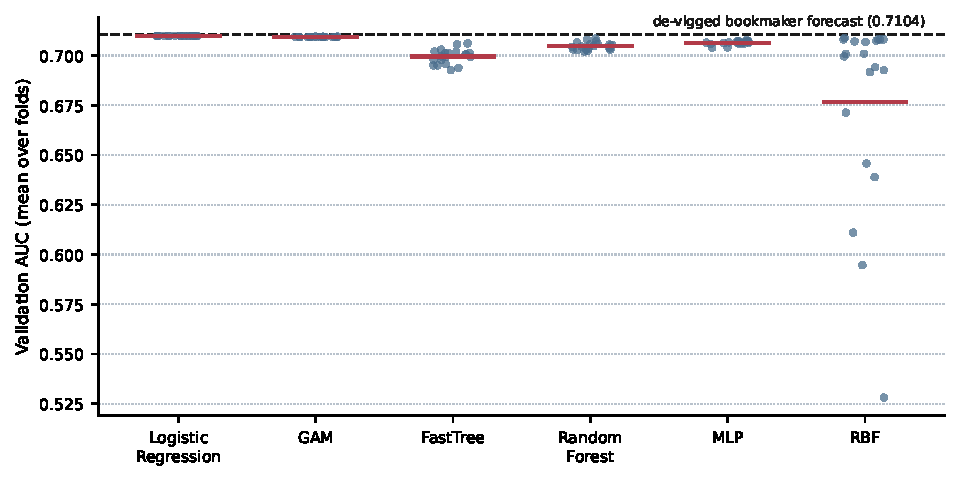
\includegraphics[width=0.95\columnwidth]{sensitivity_home}
\par\end{centering}
\caption{Hyperparameter sensitivity in the Home Win market. Each point is one
of the twenty configurations drawn for a classifier, scored by three-fold
expanding-window validation inside the training set; the horizontal
bar is the mean of the classifier and the dashed line is the de-vigged
bookmaker forecast evaluated on the same folds. The search was carried
out on the most recent 50,000 matches of the training set and the
test set was not used at any stage.\label{fig:tuning-sensitivity}}
\end{figure}


\section{Conclusions\label{sec:Conclusions}}

This study presented a unified benchmarking study for football match
outcome classification, evaluating six classifiers - Logistic Regression,
GAM, FastTree, RF, RBF, and MLP - on a large-scale dataset of 225,474
matches spanning 2018--2026. Under strictly uniform experimental
conditions the six classifiers performed almost identically. In the
Home Win market error ranged from 34.50\% to 34.73\% and macro-averaged
precision from 64.83\% to 65.16\%; in the Away Win market from 27.83\%
to 27.98\% and from 68.05\% to 68.46\% respectively. In both markets
the marginal bootstrap intervals overlap substantially, and the small
differences between the point estimates are not interpreted as evidence
of a ranking. What does separate the predictors is the comparison
with the two reference rows: every model improves clearly on the majority-class
baseline, and every model coincides with the de-vigged bookmaker forecast
to within a small fraction of a percentage point.

These results indicate that under a common experimental protocol the
choice among six established classifiers has a smaller effect on predictive
performance than the information contained in the feature set: without
odds-based inputs all six classifiers span only 0.08 accuracy points,
and 0.27 points when the odds are included. When market prices are
included among the inputs, every model reproduces the bookmaker forecast;
when market prices are excluded, the models recover approximately
half of the distance from a trivial baseline to the market (43.4\%
to 48.0\% against 51.9\% for the market). This is consistent with
earlier evidence that odds-setters are competitive forecasters in
their own right.

Several limitations should be stated. First, no model improves upon
the de-vigged bookmaker forecast on any proper scoring rule; the GAM
attains a small advantage in accuracy, which is not a proper scoring
rule and which is not accompanied by any improvement in logarithmic
loss, Brier score or the RPS, so the comparison with the market should
be read as a benchmark rather than as evidence of practical advantage.\textbf{
That advantage is the only statistically distinguishable improvement
over the market reported anywhere in this study, and it corresponds
to about 65 additional correct predictions out of 75,495.} Second,
only a single pre-match odds snapshot from one provider is available,
so neither the movement of odds between opening and closing nor the
dispersion of prices across providers - the two signals most often
associated with market inefficiency - can be examined. Third, player-level
and lineup information is not available, which restricts the feature
space to team-level aggregates. Fourth, the draw outcome is poorly
predicted both by the models and by the market (AUC 0.584), and single-threshold
measures are uninformative for it. Fifth, historical features must
be imputed for 22.4\% of matches, mainly newly promoted teams and
matches early in a season; the associated data-availability indicators
carry measurable predictive signal, but that signal reflects the composition
of the dataset rather than any footballing quantity, and a robustness
check reported in the feature-importance subsection shows that removing
them costs at most 0.22 accuracy points and leaves the conclusions
unchanged. Sixth, the analysis is confined to the pooled dataset:
per-competition modelling and cross-competition transfer were not
examined and are left for future work. Finally, probability calibration
is not addressed in this study: applying an isotonic or Platt correction
to the model outputs and testing whether it improves the probabilistic
scores reported above is left for future work.

We have not added recurrent or attention-based baselines, and the
reason is empirical rather than practical. The feature space consists
of team-level attributes summarised per match, with no sequential
or relational structure of the kind these architectures exploit. As
an additional diagnostic, a logistic regression was fitted on the
training set with the de-vigged market log-odds entered as a fixed
offset, so that the remaining standardised features could only correct
it, and the fitted correction was small. The convergence of six classifiers
of very different flexibility, reported above, points to the information
in the available features rather than model capacity as the principal
constraint, and therefore provides limited empirical motivation for
applying substantially more complex architectures to the same inputs.
We present this as an indication rather than a proof: six converging
classifiers and a small offset correction constitute strong empirical
evidence, not a demonstration that no more expressive architecture
could help.

Future work will extend the analysis to competitions modelled individually,
to the question of distribution shift between them, and to competitions
beyond those currently available, and will investigate whether league-aware
feature engineering or transfer-learning strategies are of use when
a model is confined to a single, smaller competition. Two directions
appear particularly promising: the use of odds movement and cross-provider
price dispersion, which would allow the market benchmark to be tested
rather than merely matched, and the incorporation of sequential match-event
data, for which recurrent or attention-based architectures would be
appropriate.

\vspace{6pt}


\authorcontributions{M.S. and I.G.T. conducted the experiments, using the study dataset,
and provided the comparative experiments. M.S. and G.G. performed
the statistical analysis and prepared the manuscript. All authors
have read and agreed to the published version of the manuscript.}

\funding{This research has been financed by the European Union: Next Generation
EU through the Program Greece 2.0 National Recovery and Resilience
Plan, under the call RESEARCH -- CREATE -- INNOVATE, project name
“iCREW: Intelligent small craft simulator for advanced crew training
using Virtual Reality techniques\textquotedbl{} (project code: TAEDK-06195).}

\institutionalreview{Not applicable.}

\dataavailability{The match results and pre-match odds analysed in this study were
collected from the publicly accessible OPAP-branded pages, under the
mandatory exception for text and data mining for the purposes of scientific
research (Article 21A of Law 2121/1993, as added by Law 4996/2022,
transposing Article 3 of Directive (EU) 2019/790). That exception
authorises the reproductions and extractions necessary for scientific
text and data mining and permits secure retention for research purposes,
including verification of results, but it does not itself confer a
right to redistribute the source records publicly, and the compilation
may in addition attract the sui generis database right of Article
45A of the same Law. The records are therefore not redistributed,
and neither are the de-vigged probabilities, because they remain directly
derived from the source market prices. No dataset and no code are
deposited with this article. \textcolor{Black}{What the study offers
in their place is a specification complete enough to be reimplemented
against an independently obtained source of results and prices: Section
2 states the point-in-time rule under which every historical feature
is built and the venue-specific window over which the rolling quantities
are computed, the treatment of teams without sufficient history and
the share of matches it affects, the winsorisation threshold and the
fact that it is estimated on the training period alone, the date of
the chronological split together with the resulting sample sizes,
the checks carried out for leakage between the two periods, and the
fixed hyperparameter configurations alongside the ranges over which
the sensitivity analysis was conducted.}}

\conflictsofinterest{The authors declare no conflicts of interest.}

\appendixtitles{no}

\appendix

\begin{adjustwidth}{-\extralength}{0cm}{}


\reftitle{References}
\begin{thebibliography}{99}
\bibitem[(2006)]{physics_ml1} Raissi, M., \& Karniadakis, G. E. (2018).
Hidden physics models: Machine learning of nonlinear partial differential
equations. Journal of Computational Physics, 357, 125-141.\url{https://doi.org/10.1016/j.jcp.2017.11.039}

\bibitem{physics_ml2} Kashinath, K., Mustafa, M., Albert, A., Wu,
J. L., Jiang, C., Esmaeilzadeh, S., ... \& Prabhat, N. (2021). Physics-informed
machine learning: case studies for weather and climate modelling.
Philosophical Transactions of the Royal Society A, 379(2194), 20200093.\url{https://doi.org/10.1098/rsta.2020.0093}

\bibitem[(2006)]{astronomy_ml1} Viquar, M., Basak, S., Dasgupta,
A., Agrawal, S., \& Saha, S. (2019). Machine learning in astronomy:
A case study in quasar-star classification. Emerging Technologies
in Data Mining and Information Security: Proceedings of IEMIS 2018,
Volume 3, 827-836.\url{https://doi.org/10.1007/978-981-13-1501-5_72}

\bibitem[(2006)]{astronomy_ml2} Luo, S., Leung, A. P., Hui, C. Y.,
\& Li, K. L. (2020). An investigation on the factors affecting machine
learning classifications in gamma-ray astronomy. Monthly Notices of
the Royal Astronomical Society, 492(4), 5377-5390.\url{https://doi.org/10.1093/mnras/staa166}

\bibitem[(2006)]{chemistry_ml1} Meuwly, M. (2021). Machine learning
for chemical reactions. Chemical Reviews, 121(16), 10218-10239.\url{https://doi.org/10.1021/acs.chemrev.1c00033}

\bibitem{chemistry_ml2} J.A. Aguiar, M.L. Gong, T. Tasdizen, Crystallographic
prediction from diffraction and chemistry data for higher throughput
classification using machine learning, Computational Materials Science
\textbf{173}, 109409, 2020.\url{https://doi.org/10.1016/j.commatsci.2019.109409}

\bibitem[(2006)]{med_ml1} S.S. Yadav, S.M. Jadhav, Deep convolutional
neural network based medical image classification for disease diagnosis.
J Big Data \textbf{6}, 113, 2019.\url{https://doi.org/10.1186/s40537-019-0276-2}

\bibitem{med_ml2} L. Qing, W. Linhong, D. Xuehai, A Novel Neural
Network-Based Method for Medical Text Classification, Future Internet
\textbf{11}, 255, 2019. \url{https://doi.org/10.3390/fi11120255}

\bibitem[(2006)]{econ_ml1} Athey, S. (2018). The impact of machine
learning on economics. In The economics of artificial intelligence:
An agenda (pp. 507-547). University of Chicago Press.\url{https://doi.org/10.7208/chicago/9780226613475.003.0021}

\bibitem{econ_ml2} R. Hafezi, J. Shahrabi, E. Hadavandi, A bat-neural
network multi-agent system (BNNMAS) for stock price prediction: Case
study of DAX stock price, Applied Soft Computing \textbf{29}, pp.
196-210, 2015.\url{https://doi.org/10.1016/j.asoc.2014.12.028}

\bibitem{nn_image} Ghai, D., Tripathi, S. L., Saxena, S., Chanda,
M., \& Alazab, M. (Eds.). (2022). Machine learning algorithms for
signal and image processing. John Wiley \& Sons.\url{https://doi.org/10.1002/9781119861850}

\bibitem{nn_timeseries} Ahmed, N. K., Atiya, A. F., Gayar, N. E.,
\& El-Shishiny, H. (2010). An empirical comparison of machine learning
models for time series forecasting. Econometric reviews, 29(5-6),
594-621.\url{https://doi.org/10.1080/07474938.2010.481556}

\bibitem[(2009)]{nn1} Zou, J., Han, Y., \& So, S. S. (2009). Overview
of artificial neural networks. Artificial neural networks: methods
and applications, 14-22.\url{https://doi.org/10.1007/978-1-60327-101-1_2}

\bibitem[(2009)]{nn2} Abiodun, O. I., Jantan, A., Omolara, A. E.,
Dada, K. V., Mohamed, N. A., \& Arshad, H. (2018). State-of-the-art
in artificial neural network applications: A survey. Heliyon, 4(11).\url{https://doi.org/10.1016/j.heliyon.2018.e00938}

\bibitem[(2009)]{dt1} De Ville, B. (2013). Decision trees. Wiley
Interdisciplinary Reviews: Computational Statistics, 5(6), 448-455.\url{https://doi.org/10.1002/wics.1278}

\bibitem[(2009)]{dt2} Kotsiantis, S. B. (2013). Decision trees: a
recent overview. Artificial Intelligence Review, 39(4), 261-283.\url{https://doi.org/10.1007/s10462-011-9272-4}

\bibitem[(2009)]{svm1} Pisner, D. A., \& Schnyer, D. M. (2020). Support
vector machine. In Machine learning (pp. 101-121). Academic Press.\url{https://doi.org/10.1016/b978-0-12-815739-8.00006-7}

\bibitem[(2009)]{svm2} Valkenborg, D., Rousseau, A. J., Geubbelmans,
M., \& Burzykowski, T. (2023). Support vector machines. American journal
of orthodontics and dentofacial orthopedics, 164(5), 754-757.\url{https://doi.org/10.1016/j.ajodo.2023.08.003}

\bibitem{power} Clarke, S. (2016). A review of methods for deriving
probability estimates from betting odds.

\bibitem{gam} Wood, S. N. (2017). Generalized Additive Models: An
Introduction with R (2nd ed.). Chapman and Hall/CRC.\url{https://doi.org/10.1201/9781315370279}

\bibitem[(2017)]{fasttree}\textbf{Friedman, J. H. (2001). Greedy
function approximation: a gradient boosting machine. Annals of Statistics,
29(5), 1189-1232.}\url{https://doi.org/10.1214/aos/1013203451}

\bibitem{randomForest} Liaw, A., \& Wiener, M. (2002). Classification
and regression by random Forest. R News, 2(3), 18-22.

\bibitem[(2009)]{elo_football} Hvattum, L. M., \& Arntzen, H. (2010).
Using ELO ratings for match result prediction in association football.
International Journal of forecasting, 26(3), 460-470.\url{https://doi.org/10.1016/j.ijforecast.2009.10.002}

\bibitem[(2009)]{ml_bayesian} Marcot, B. G., \& Penman, T. D. (2019).
Advances in Bayesian network modelling: Integration of modelling technologies.
Environmental modelling \& software, 111, 386-393.\url{https://doi.org/10.1016/j.envsoft.2018.09.016}

\bibitem[(2009)]{bayesian_football} Owramipur, F., Eskandarian, P.,
\& Mozneb, F. S. (2013). Football result prediction with Bayesian
network in Spanish League-Barcelona team. International Journal of
Computer Theory and Engineering, 5(5), 812.\url{https://doi.org/10.7763/ijcte.2013.v5.802}

\bibitem[(2009)]{ml_logistic} Stoltzfus, J. C. (2011). Logistic regression:
a brief primer. Academic emergency medicine, 18(10), 1099-1104.\url{https://doi.org/10.1111/j.1553-2712.2011.01185.x}

\bibitem[(2009)]{logistic_football} D. Prasetio and D. Harlili, \textquotedbl Predicting
football match results with logistic regression,\textquotedbl{} 2016
International Conference On Advanced Informatics: Concepts, Theory
And Application (ICAICTA), Penang, Malaysia, 2016, pp. 1-5, doi: 10.1109/ICAICTA.2016.7803111.\url{https://doi.org/10.1109/icaicta.2016.7803111}

\bibitem[(2009)]{polynomial_football} Martins, R. G., Martins, A.
S., Neves, L. A., Lima, L. V., Flores, E. L., \& do Nascimento, M.
Z. (2017). Exploring polynomial classifier to predict match results
in football championships. Expert Systems with Applications, 83, 79-93.\url{https://doi.org/10.1016/j.eswa.2017.04.040}

\bibitem[(2009)]{rf_football} Schauberger, G., \& Groll, A. (2018).
Predicting matches in international football tournaments with random
forests. Statistical Modelling, 18(5-6), 460-482.\url{https://doi.org/10.1177/1471082x18799934}

\bibitem[(2009)]{attr_football} Danisik, N., Lacko, P., \& Farkas,
M. (2018, August). Football match prediction using players attributes.
In 2018 World symposium on digital intelligence for systems and machines
(DISA) (pp. 201-206). IEEE.\url{https://doi.org/10.1109/disa.2018.8490613}

\bibitem[(2009)]{dolores_football} Constantinou, A. C. (2019). Dolores:
a model that predicts football match outcomes from all over the world.
Machine learning, 108(1), 49-75.\url{https://doi.org/10.1007/s10994-018-5703-7}

\bibitem[(2009)]{ml_boosting} Natekin, A., \& Knoll, A. (2013). Gradient
boosting machines, a tutorial. Frontiers in neurorobotics, 7, 63623.\url{https://doi.org/10.3389/fnbot.2013.00021}

\bibitem[(2009)]{boost_football} Baboota, R., \& Kaur, H. (2019).
Predictive analysis and modelling football results using machine learning
approach for English Premier League. International Journal of Forecasting,
35(2), 741-755.\url{https://doi.org/10.1016/j.ijforecast.2018.01.003}

\bibitem[(2009)]{deep_football} Rahman, M. A. (2020). A deep learning
framework for football match prediction. SN Applied Sciences, 2(2),
165.\url{https://doi.org/10.1007/s42452-019-1821-5}

\bibitem[(2008)]{rff} A. Rahimi and B. Recht, Random features for
large-scale kernel machines, Advances in Neural Information Processing
Systems 20, pp. 1177-1184, 2008.

\bibitem{forrest2005}\textbf{Forrest, D., Goddard, J., \& Simmons,
R. (2005). Odds-setters as forecasters: The case of English football.
International Journal of Forecasting, 21(3), 551-564.\url{https://doi.org/10.1016/j.ijforecast.2005.03.003}}

\bibitem{dixoncoles1997}\textbf{Dixon, M. J., \& Coles, S. G. (1997).
Modelling association football scores and inefficiencies in the football
betting market. Journal of the Royal Statistical Society: Series C,
46(2), 265-280.\url{https://doi.org/10.1111/1467-9876.00065}}

\bibitem{gneiting2007}\textbf{Gneiting, T., \& Raftery, A. E. (2007).
Strictly proper scoring rules, prediction, and estimation. Journal
of the American Statistical Association, 102(477), 359-378.\url{https://doi.org/10.1198/016214506000001437}}

\bibitem{wheatcroft2021}\textbf{Wheatcroft, E. (2021). Evaluating
probabilistic forecasts of football matches: the case against the
ranked probability score. Journal of Quantitative Analysis in Sports,
17(4), 273-287.\url{https://doi.org/10.1515/jqas-2019-0089}}

\bibitem{constantinou2012}\textbf{Constantinou, A. C., \& Fenton,
N. E. (2012). Solving the problem of inadequate scoring rules for
assessing probabilistic football forecast models. Journal of Quantitative
Analysis in Sports, 8(1).\url{https://doi.org/10.1515/1559-0410.1418}}

\bibitem{efron1993}\textbf{Efron, B., \& Tibshirani, R. J. (1993).
An Introduction to the Bootstrap. Chapman \& Hall/CRC.}

\bibitem{kliger2025}\textbf{Kliger, D., Mugerman, Y., \& Rooz, R.
(2025). Eponymy family firms and optimistic forecasts. Finance Research
Letters, 85, Article 108032.\url{https://doi.org/10.1016/j.frl.2025.108032}}

\end{thebibliography}
%%%%%%%%%%%%%%%%%%%%%%%%%%%%%%%%%%%%%%%%%%
%% for journal Sci
%\reviewreports{\\
%Reviewer 1 comments and authors' response\\
%Reviewer 2 comments and authors' response\\
%Reviewer 3 comments and authors' response
%}
%%%%%%%%%%%%%%%%%%%%%%%%%%%%%%%%%%%%%%%%%%

\PublishersNote{}

\end{adjustwidth}{}
\end{document}
